%--------------------------------------------------------%
% Journal Article Manuscript Template
%--------------------------------------------------------%

% GENERAL MANUSCRIPT TEMPLATE

	% by Nicholas E. Reith

	% DATE: November 26th, 2014

%--------------------------------------------------------%
%	PREAMBLE
%--------------------------------------------------------%

% DOCUMENT CLASS
    % Change "letterpaper" to "a4" if you use a4 paper size
    \documentclass[letterpaper,12pt]{article}
  
% TITLE SECTION
	
 %Abstract
    \usepackage{abstract} % Allows abstract customization
    % Set the "Abstract" text to bold
    \renewcommand{\abstractnamefont}{\normalfont\bfseries}
    % Set the abstract itself to small italic text
    \renewcommand{\abstracttextfont}{\normalfont\small\itshape} 

 %Title
    \usepackage{titlesec} % Allows customization of titles

 %Authors
    \usepackage{authblk} % For multiple authors

 %Date
	\usepackage{datetime} % allows for including today's date
  	% These two lines creates a new date format ``Month day(th), year''
    \newdateformat{usvardate}{
  	\monthname[\THEMONTH] \ordinal{DAY}, \THEYEAR}

% HEADERS & FOOTERS

 %Footnotes
  	\usepackage[bottom]{footmisc} % Makes footnotes stick to bottom of the page
    
 %Endnotes
	% Uncomment this line if using endnotes "\endnote{}"
	% \usepackage{endnotes}
    
 %Headers from page 2 on
    \usepackage{fancyhdr}
    \pagestyle{fancy}
    \fancyheadoffset{0cm}
    \setlength{\headheight}{15pt} 
 
% DRAFT WATERMARK
	% NOTE: Comment out these two lines to remove watermark
    \usepackage[firstpage]{draftwatermark} % adds draft watermark
    \SetWatermarkLightness{0.85}

% MACROS
    % Define keywords macro command
    \providecommand{\keywords}[1]{\textbf{\textit{Keywords---}} #1}

%% LianTze 7 Dec 2016:
%% Updated how the wordcount is implemented
\newcommand\wordcount{%
  \immediate\write18{texcount -utf8 -merge -sum -incbib -dir -sub=none -brief \jobname.tex | cut -d : -f 1 > 'count.txt'}%
  \input{count.txt}\ignorespaces words%
}
  

% MATH SUPPORT
    % The amssymb package provides various useful mathematical symbols
    \usepackage{amssymb}
    % The amsthm package provides extended theorem environments
    \usepackage{amsthm}
    % The newtxmath package provides additional math symbol support
    	% in Times New Roman symbols, etc.
    \usepackage{newtxmath}

% FONTS
    \usepackage{microtype} % Slightly tweak font spacing for aesthetics
    \usepackage[utf8]{inputenc}
    \usepackage{newtxtext} % Makes default font Adobe Times New Roman
  
% LINES
	% Spacing
	\usepackage{setspace} % See \doublespacing command at the top of content.tex
    % Numbering
    \usepackage{lineno,xcolor} 	% See \linenumbers at the top of content.tex

% MARGINS
	%NOTE: All spaces in this template are in inches, because it is
    % formatted for letterpaper (8.5 x 11 inch) paper. If you use a4
    % paper, choose different sizes in millimeters or centimeters.
	\usepackage[top=1.5in, bottom=1.5in, left=1in, right=1in]{geometry}

% COMMENTS
	\usepackage[colorinlistoftodos]{todonotes} % allows margin comments
    % See examples in content.tex, and here for manual: 
    % http://www.ctan.org/pkg/todonotes
	\usepackage{soul} % allows for highlighting
    
% GRAPHICS
    \usepackage{graphicx} % More advanced figure inclusion
    \usepackage{float} % For specifying table/figure locations, i.e. [ht!]
    
    % The printlen command allows the user to print the exact text width or height.
    % This is useful, when trying to create graphics (outside of LaTeX, of course)
    % with the optimal dimensions. See here for usage: http://www.ctan.org/pkg/printlen
    \usepackage{printlen}

% TABLES
    \usepackage{longtable} % For long tables that span multiple pages
    \newcommand{\sym}[1]{\rlap{#1}}% For symbols like *** in tables
    \usepackage{tabularx} % Allows advanced table features
    \newcolumntype{L}[1]{>{\raggedright\arraybackslash}p{#1}}
    \newcolumntype{C}[1]{>{\centering\arraybackslash}p{#1}}
    \newcolumntype{R}[1]{>{\raggedleft\arraybackslash}p{#1}}
    \usepackage{relsize} % Allows precise adjustment of font size,
    	%useful for fitting tables to page width

% REFERENCES
	\usepackage{hyperref} % For hyperlinks in the PDF

      % NOTE: This document uses bibtex for references
      % because both style files for Sociology Journals are
      % only available in .bst format. You can change to
      % biblatex if you prefer below.

      % Many thanks to Sociology Professor, 
      % ChangHwan Kim at the University of Kansas. 
      % for providing these .bst files here: 
      % http://people.ku.edu/~chkim
      
	% BIBTEX
    % Comment out this line if using biblatex
    \usepackage{chicago} % AJS and ASR styles rely on chicago

    % BIBLATEX
    % NOTE: Uncomment out these three lines to use biblatex
    % Be sure to put the biblio.bib file in biblatex format'
    %\usepackage{csquotes}
	%\usepackage[style=authoryear,backend=biber]{biblatex}
	%\bibliography{biblio}
    
 % Edit preamble.tex to change the overall layout

% Header from Page Three on: Edit below for left and right headers
\lhead{}
\rhead{}

%--------------------------------------------------------%
% BEGIN DOCUMENT
%--------------------------------------------------------%

\begin{document}

% COVER PAGE

%!TEX root = ../main.tex

\begin{titlepage}

  \newcommand{\HRule}{\rule{\linewidth}{0.5mm}} % Defines a new command for the horizontal lines, change thickness here

  \center % Center everything on the page


% HEADING SECTION

  %\textsc{\LARGE University Name}\\[1.5cm] % Name of your university/college
  % \textsc{\Large Manuscript Submission}\\[0.5cm] % Major heading such as course name
  % \textsc{\large The Journal of Blah Blah}\\[0.5cm] % Minor heading such as course title

% TITLE SECTION

  \vspace{3.5 cm}
  { \huge \bfseries Correlating Microbial Abundances for the Microbial Interaction Network Database}\\[0.4cm] % Title of your document

% AUTHOR SECTION

  \vspace{1.5 cm}
  Dileep Kishore, Gabriel Birzu, Zhenjun Hu, Charles DeLisi, Kirill Korolev, Daniel Segre\\
  \vspace{1cm}
  Department of XYZ,\\
  The University of ABC\\
  Department of ABC,\\
  XYZ University\\

% DATE SECTION

  % \vspace{1.5 cm}
  % {\large Submitted: \today}\\[3cm] % Date, change the \today to a set date if you want to be precise


\vfill % Fill the rest of the page with whitespace

\end{titlepage}

%-----------------------------------------------------------------

\newpage
 % Comment out to remove cover page

\thispagestyle{empty} % Removes header on page two.

% NOTE: Comment out the lines below to remove line numbers
  % Running line numbers:
  \linenumbers
  \setlength\linenumbersep{15pt}
  \renewcommand\linenumberfont{\normalfont\footnotesize\sffamily\color{gray}}
  %\pagewiselinenumbers % Same, but that reset on every page:
  \modulolinenumbers[1] % Number only every line. Change for fewer.

%--------------------------------------------------------%
%   CONTENT
%--------------------------------------------------------%

% ABSTRACT
%!TEX root = ../main.tex

\begin{abstract}
  {
    \noindent
    Microbes tend to organize into communities consisting of hundreds of species involved in complex interactions with each other.
    16S ribosomal RNA (16S rRNA) amplicon profiling provides snapshots that reveal the phylogenies and abundance profiles of these microbial communities.
    These snapshots, when collected from multiple samples, have the potential to reveal which microbes co-occur, providing a glimpse into the network of associations in these communities.
    The inference of networks from 16S data is prone to statistical artifacts.
    There are many tools for performing each step of the 16S analysis workflow, but the extent to which these steps affect the final network is still unclear.
    In this study, we perform a meticulous analysis of each step of a pipeline that can convert 16S sequencing data into a network of microbial associations.
    Through this process, we map how different choices of algorithms and parameters affect the co-occurrence network and estimate steps that contribute most significantly to the variance. We further determine the tools and parameters that generate the most accurate and robust co-occurrence networks based on comparison with mock and synthetic datasets.
    Ultimately, we develop a standardized pipeline (available at \href{https://github.com/segrelab/MiCoNE}{https://github.com/segrelab/MiCoNE}) that follows these default tools and parameters, but that can also help explore the outcome of any other combination of choices.
    We envisage that this pipeline could be used for integrating multiple data-sets, and for generating comparative analyses and consensus networks that can help understand and control microbial community assembly in different biomes.
}  
\end{abstract}

% Insert keywords here
\keywords{Microbiome, 16S rRNA, Pipeline, Interaction, Denoising, Taxonomy, Network Inference, Correlations, Qiime, Co-occurrence, Networks}


\section*{Importance}
  
To understand and control the mechanisms that determine the structure and function of microbial communities, it is important to map the interrelationships between its constituent microbial species. The surge in the high-throughput sequencing of microbial communities has led to the creation of thousands of datasets containing information about microbial abundances. These abundances can be transformed into networks of co-occurrences across multiple samples, providing a glimpse into the structure of microbiomes. However, processing these datasets to obtain co-occurrence information relies on several complex steps, each of which involves multiple choices of tools and corresponding parameters. These multiple options pose questions about the accuracy and uniqueness of the inferred networks. In this study, we address this workflow and provide a systematic analysis of how these choices of tools and parameters affect the final network, and on how to select those that are most appropriate for a particular dataset.

\doublespacing

% INTRODUCTION
%!TEX root = ../main.tex

\section*{Introduction}

  Microbial communities are ubiquitous and play an important role in biogeochemical transformations in both natural as well as man-made ecosystems.
  These microbiomes comprise several thousand different microbial strains interacting with each other and their environment, often through intricate metabolic and signaling relationships.
  Changes in the microbiome can alter the environment in which they reside \cite{HumanMicrobiomeProjectConsortium2012,Lloyd-Price2016} and for host-associated microbiomes this can have major implications in health of the human body.
  A mechanistic understanding of the key interactions between microbes is necessary in order to analyze the dysbiosis in a healthy microbiome and to design interventions.

  Studies have shown the importance of specific microbial interactions in the healthy microbiome \cite{Lloyd-Price2016} and others have shown how changes in these interactions can lead to dysbiosis \cite{Wang2017,Gilbert2016,Belizario2015}.
  While direct measurement of interactions is challenging, a significant amount of effort has gone into measuring correlations leading to the correlation information between microbial abundances being readily available.
  Co-occurrence relationships in microbial communities may be driven by microbial interactions, although the extent and nature of these relationships is highly debated \cite{Zuniga2017}.
  Each interaction within this complex ecological network can have a positive effect, a negative effect or no effect on the species involved.
  Bacteria that compete for the same nutrient will have a negative co-occurrence relationship \cite{Ghoul2016} whereas cross-feeding between species leads to a positive co-occurrence relationship \cite{DSouza2018}.
  But these co-occurrence relationships are not very straightforward, since, similar species competing for a resource could co-occur if the resource is abundant.
  The microbial interaction networks are highly dynamic, and they constantly reorganize in a varying environment.
  Even under static conditions, these interactions are often difficult to predict due to their non-linear nature \cite{Konopka2015}.
  Compounding on this complexity is the fact that these interaction networks usually involve thousands of species.

  High-throughput metagenomic sequencing techniques (such as 16S rRNA gene profiling) help detect, identify and quantify a large part of the constitutive microorganisms of a microbiome \cite{Jovel2016}.
  Knowledge of the community composition at a particular instance in time would enable us to derive partial insights into the underlying dynamics.
  With the advancement in DNA sequencing technologies \cite{Narihiro2017} and data processing methods much more information can be extracted from these microbial community samples than ever before.
  These advances have led to large-scale data collection efforts involving environmental (Earth Microbiome Project) \cite{Thompson2017}, marine (Tara Oceans Project) \cite{Zhang2015} and human-associated microbiota (Human Microbiome Project) \cite{HumanMicrobiomeProjectConsortium2012} and thus led the generation of a wealth of data about these microbial communities.
  
  These data-sets can be used to infer networks of co-occurrence relationships between microorganisms in the samples.
  These networks have microbial taxa as nodes, and edges that represent the frequent co-occurrence (or negative correlations) across different datasets.
  Co-occurrence networks can in principle be used to identify important interactions driving the dynamics of the microbial community, including emergent ecosystem-level properties such as ecosystem robustness and modularity.

  One of the limitations of this type of analysis is that 16S sequencing data is limited by many factors such as resolution, sequencing depth, compositional nature, sequencing errors and copy number variations.
  Many different analysis methods have been developed \cite{Callahan2016,Amir2017,Friedman2012,Kurtz2015} to counter these limitations and remove statistical artifacts, leading to the existence of a myriad of tools for each step of the data analysis workflow.
  The different methods and tools developed to solve these issues infer vastly different community compositions and co-occurrence networks \cite{Golob2017,Weiss2016}, making it difficult to reliably compare networks across different publications and studies.
  Conversely, given the lack of comprehensive comparisons between directly observed microbial interactions (e.g. from co-culture experiments) and co-occurence networks, there is no straightforward way to determine which set of tools or methods generate the most accurate networks.
  
 Previous work has developed popular platforms (like MG-RAST \cite{Keegan2016}, Qiita \cite{qiita}) and tools (such as QIIME \cite{Caporaso2010}) that provide pipelines for 16S data analysis. However, existing tools typically are not focused on the effects of upstream statistical methods on the inferred co-occurrence networks. Furthermore, no organized framework currently exist to systematically analyze and compare existing components of the data-analysis from amplicons to networks.
  
  In this study, we present a standardized 16S data-analysis pipeline called \ac{micone} that produces robust and reproducible co-occurrence networks from community 16S sequence data, and allow users to interactively explore how the network would change upon using different alternative tools and parameters at each step.
  % TODO: Link or describe MIND here
  Our pipeline is coupled to an online integrative tool for the organization, visualization and analysis of inter-microbial networks.
  In addition to making this tool freely available, we implemented a systematic comparative analysis to determine which steps of the pipeline have the largest influence on the final network, and what choice seems to provide best agreement with the tested mock and synthetic datasets.
  We believe that these steps will ensure better reproducibility and easier comparison of co-occurrence networks across data-sets.
  We expect that our tool will also be useful for benchmarking future alternative methods, and for ensuring a transparent evaluation of the possible biases introduced by the use of specific tools.


% RESULTS
%!TEX root = ../main.tex

\section*{Results}

  \subsection*{\acl{micone} (\acs{micone})}

  We developed \ac{micone}, a flexible and modular pipeline for the inference of co-occurrence networks from 16S data.
  \ac{micone} incorporates various popular, publicly available tools as well as custom Python modules for 16S data analysis and network inference (Methods).
  The different steps that are a part of the \ac{micone} co-occurrence network inference workflow (Figure~\ref{fig:figure1}) can be grouped into five major modules; (i) \ac{sp}; (ii) \ac{dc}; (iii) \ac{ta}; (iv) \ac{op}; and (v) \ac{ni}.
  Each process in the pipeline is implemented through multiple tools (see Methods and Figure~\ref{fig:figure1}).
  The effects of changing any intermediate step of the pipeline can be evaluated in terms of the final network outcome, as well as on any of the intermediate metrics and data outputs.
  The choice of tools and parameters is encoded in a configuration file (with parameters as shown in Tables S2-S6 at \href{https://github.com/segrelab/MiCoNE-pipeline-paper}{https://github.com/segrelab/MiCoNE-pipeline-paper}).
  Through a systematic analysis of tool combinations at each step of the pipeline, we estimated how much the final co-occurrence network depends on the possible choices at each step.

  Our analysis involved two types of data: The first type consisted of 16S sequencing data from samples of human stool microbiomes from a fecal microbiome transplant (FMT) study of autism~\cite{Kang2017}.
  The second type was a collection of datasets synthetically or artificially created for the specific goal of evaluating computational analysis tools.
  In particular, in order to benchmark each step in \ac{micone}, we used both mock data (labeled mock4, mock12, and mock16) from mockrobiota~\cite{Bokulich2016} and synthetic networks generated using the NorTA~\cite{Kurtz2015} and seqtime~\cite{Rottjers2018} approaches (See Methods).

  \FloatBarrier

  \subsection*{DC: Denoising and clustering methods differ in their identification of sequences that are low in abundance}

  The \ac{dc} step is commonly carried out to generate representative sequences (in the form of the \acs{otu}/\acs{esv} tables) from the demultiplexed and trimmed 16S sequencing data.
  In order to compare the count tables generated by different tools, we processed the 16S sequencing reads (from the FMT study~\cite{Kang2017}) using 5 different methods: open-reference clustering, closed-reference clustering, de novo clustering, \ac{dada2}~\cite{Callahan2016} and Deblur~\cite{Amir2017}.
  The first three methods are from the vsearch plugin from \ac{qiime2}~\cite{bolyenReproducibleInteractiveScalable2019}.
  The closed and open reference methods in this analysis use the \acl{gg}~\cite{DeSantis2006} database for reference sequence alignment.

  A comparison of the different methods was carried out by calculating the mean UniFrac distances across all samples (Figure~\ref{fig:figure2}).
  The analysis was performed using both the weighted UniFrac~\cite{Lozupone2007} (Figure~\ref{fig:figure2}A) distance metric, which takes into account the counts of the representative sequences, and the unweighted UniFrac~\cite{Lozupone2005} (Figure~\ref{fig:figure2}B) distance metric, which gives equal weights to each sequence.

  The first main message emerging from this analysis is that the representative sequences generated by the different methods, with the exception of Deblur, are similar to each other when weighted by their abundance (Figure~\ref{fig:figure2}A).
  A second message is that the different methods differ mainly in the assignment of sequences of lower abundance.
  This can be inferred from the unweighted comparison (Figure~\ref{fig:figure2}B) which shows an increase in dissimilarity between each pair of methods (see additional details in Supplementary and Figure \ref{fig:figure_s2}).

  These comparisons only elucidate the similarity between a pair of methods.
  To determine which tool most accurately recapitulates the reference sequences in the samples, we applied the same pipeline step to process the mock datasets (mock4, mock12, and mock16) and compared the predicted representative sequences with the true sequences and their distribution.
  The results (Figure~\ref{fig:figure2}C and \ref{fig:figure2}D) show that the predicted sequence distributions are overall different from the expected ones.
  The variation across datasets indicates that the datasets themselves play a big role in method performance.
  We note that there is no method that outperforms the rest in all datasets (see Supplementary for an extended discussion).
  Based on their slightly better performance on the mock datasets, their de novo error correcting nature and previous independent evaluation~\cite{Nearing2018}, \ac{dada2} and Deblur appear to be the most reliable.
  This is because the open-reference and de novo clustering methods return a much larger number of \ac{otu}s compared to the other pipelines and would affect the accuracy of the network inference step if stringent filtering is not performed.
  Overall, since \ac{dada2} as compared to Deblur, displays better performance on all the mock datasets on the weighted UniFrac metric, we set this tool as the default for the DC step of the pipeline.
  However, if comparison across studies that have sequenced different 16S regions is required, closed-reference and open-reference might be a better option.

  After the denoising, the sequences are subject to Chimera Checking (CC).
  The \ac{micone} pipeline supports two different chimera checking methods, ``uchime-denovo"~\cite{bolyenReproducibleInteractiveScalable2019}, and ``remove bimera"~\cite{Callahan2016}.
  We did not notice any notable difference between the two methods (Figure~\ref{fig:figure_s3}), implying that they identify and remove mostly the same set of sequences as chimeras.
  Since the remove bimera method was originally developed in conjunction with dada2 we use this method as the default.
  The DC step thus results in a reduced set of unique sequences, which will be referred to as representative sequences in the subsequent steps.

  \FloatBarrier

  \subsection*{TA: Taxonomy databases vary widely in taxonomy assignments beyond Order level}

  Taxonomy databases are used to assign taxonomic identities to the representative sequences obtained after the DC step.
  The three 16S taxonomic reference databases used in this study are SILVA~\cite{Quast2012}, \ac{gg}~\cite{DeSantis2006} and \ac{ncbi} RefSeq~\cite{Sayers2009} (Methods).
  These databases vary substantially in terms of taxonomy hierarchies, including species names and phylogenetic relationships~\cite{Balvociute2017}.
  Assignment using a particular database also requires a query tool.
  We used the ``Naive Bayes'' classifier from \ac{qiime2} for the \ac{gg} and SILVA databases and the ``BLAST'' tool (included as a \ac{qiime2} plugin) for the \ac{ncbi} database.
  These tools have been well quantified and optimized~\cite{bokulichOptimizingTaxonomicClassification2018}, hence, we made use of the default parameters in our analyses.

  The representative sequences obtained using the default settings of the DC step were used for taxonomic assignment using the three reference databases.
  Figure~\ref{fig:figure3}A depicts a flow diagram that shows how the top 50 representative sequences (sorted by abundance) are assigned a Genus according to the three databases.
  The different databases lead to assignments that qualitatively display similar distributions. However, the assigned Genus compositions also display clear differences, as does the percentage of unassigned representative sequences (pink).
  Some of the differences in Genus composition have a clear explanation, for example, abundant Genera like Bacteroides and Escherichia are assigned to different representative sequences.
  The large percentage of unassigned sequences is due to the large fraction of the representative sequences assigned to an "unknown" Genus during the assignment process (Methods).

  After the assignment, we performed a pairwise comparison of the similarity between the top 100 assignments (by abundance) from different databases at every taxonomic level (Figure~\ref{fig:figure3}B).
  The comparisons of the assignments below the Order level (Family, Genus, and Species) show less than $45\%$ similarity between any pair of databases.
  This implies that the taxonomy assignments from each reference database are fairly unique.
  The comparison of all assigned genera (Figure~\ref{fig:figure_s4}), instead of just the top 100, contains a higher percentage of mismatches.
  This suggests that, comparatively, the most abundant sequences are more consistently matched to the same taxonomies, at least for the dataset tested in the current analysis.

  To obtain an absolute measure of the accuracy of the taxonomic assignments, we used the representative sequences from the DC step for mock datasets as the query sequences and the expected taxonomic composition as the standard to compare against.
  We used the Bray-Curtis distance metric~\cite{virtanenSciPyFundamentalAlgorithms2020} to calculate the distance between the predicted and expected taxonomic distribution (Figure~\ref{fig:figure3}C).
  We find that none of the databases perform better than the others in absolute terms and that the dissimilarity with the expected composition is high ($>0.5$ for Family and Genus and $>0.9$ for Species), indicating that all the databases have some limitations when trying to recapture the expected taxonomic composition.

  Since no database performs better than others against mock datasets, the choice of which database to use could be driven by other reasons (see Supplementary discussion).
  One reason to choose a particular database could be the frequency of updates and the potential for future growth.
  Both \ac{gg}, due to its frequent use in the literature~\cite{Balvociute2017}, and \ac{ncbi}, due to its regular revision and maintenance, could be good choices for taxonomy assignment.
  In our default pipeline, we choose \ac{gg} as the default method.

  The TA step results in a taxonomic counts table that is used as input to the subsequent steps of the pipeline.
  Note that the count tables at different levels can be obtained through aggregation; for example, Genus count tables were obtained by summing up the counts of the lower taxonomy levels (Species and \ac{otu}) that map to the same higher taxonomy level entity.

  \FloatBarrier

  \subsection*{NI: Different network inference methods drastically affect edge-density and connectivity}

   The ten network inference methods we used in this step fall into two groups: the first set of methods (Pearson, Spearman, \acs{sparcc}~\cite{Friedman2012,Watts2018}, and propr~\cite{quinnProprRpackageIdentifying2017}) infer pairwise correlations while the second set (\acs{spieceasi}~\cite{Kurtz2015}, FlashWeave~\cite{tackmannRapidInferenceDirect2019}, \acs{cozine}~\cite{haCompositionalZeroinflatedNetwork2020a}, \acs{harmonies}~\cite{jiangHARMONIESHybridApproach2020}, \acs{spring}~\cite{yoonMicrobialNetworksSPRING2019}, and \acs{mldm}~\cite{Yang2017}) infer direct associations.
   Note that while Pearson and Spearman methods are included in the pipeline for completeness, they tend to generate a large number of spurious edges as they are not intended for compositional datasets.
   Thus, they are not included in subsequent quantitative analyses.

  Filtered (see \ac{op} step in Methods) genus-level counts table obtained using the default settings in the previous steps were used as input for the different network inference algorithms (Figure~\ref{fig:figure4}).
  Even from a visual inspection (Figure~\ref{fig:figure4}A), one can see that the different networks differ vastly in their edge-density and connectivity, with common edges often displaying inverted signs.

  To quantify the differences between the networks, we analyzed the distribution of common nodes and edges (Figure~\ref{fig:figure4} B and \ref{fig:figure4}C) using UpSet plots~\cite{lexUpSetVisualizationIntersecting2014}.
  The node intersection analysis shows that the networks have $33$ out of $68$ total unique nodes in common and that no network possesses a unique node.
  Edge intersections in contrast show that only $8$ edges (out of $202$ total unique edges) are in common between all the methods and each network has many unique edges.
  These results showed a substantial rewiring of connections in different inferred networks and prompted us to identify associations robust across methods, through consensus algorithms.

  \FloatBarrier

  \subsection*{NI: The scaled-sum consensus method shows high precision on benchmark datasets}

 Inspired by previous approaches~\cite{bustinceFuzzySetsTheir2008,tsarevApplicationMajorityVoting2018}, we developed two methods that take into consideration the evidence offered by each network inference algorithm and generate a consensus network that contains the common edges among the inferred networks.

  Both of our approaches - simple voting (SV) and scaled-sum (SS) - combine appropriately filtered networks inferred from correlation-based and direct association methods (see Methods).
  We chose the scaled-sum method as the pipeline default since this method takes into account the weights of the associations in the determination of the final consensus.
  The pipeline enables the selection of any subset of methods for the consensus calculation. Currently, by default, all direct methods are used, together with \acs{sparcc} and propr.

  Similar to what was done for the previous steps of the pipeline, and in analogy with previous estimations of network inference accuracy~\cite{Kurtz2015,Weiss2016}, we evaluated the network inference algorithms and the final consensus network using synthetic interaction data.
  For this purpose, we generated synthetic interaction data using the ``NorTA''~\cite{Kurtz2015} and ``seqtime''~\cite{faustSignaturesEcologicalProcesses2018} methods (see Methods).
  For each method, an \ac{otu} counts table was generated based on the selected parameters and abundance distributions.
  This counts table was used as the input to the \ac{micone} pipeline to generate predicted associations.
  The interaction network used to generate the counts table was used as the source of true interactions to calculate the precision (Figure \ref{fig:figure5}) and sensitivity (Figure \ref{fig:figure_s5} and Figure \ref{fig:figure_s6}) for each network inference algorithm.
  As shown in Figure \ref{fig:figure5} the consensus algorithm, especially the scaled-sum method, captures true associations with high precision (through the removal of edges that are either not present in most of the inference methods or whose association strength is low across methods).
  Overall, the scaled-sum method for $p=1.000$ performs the best (precision = $1.000$ for both NorTA and seqtime).
  The scaled-sum method for $p=0.333$ (default option in the pipeline) shows a high precision ($0.956$ with NorTA; $0.688$ with seqtime), without displaying significant reduction in sensitivity (Figure~\ref{fig:figure_s5} and Figure~\ref{fig:figure_s6}).
  However, if higher precision is required $p>0.5$ can be considered.
  Therefore, the consensus networks provide the means to obtain a short list of associations that would have a high likelihood of being present in the real association network.

  \FloatBarrier

  \subsection*{Impact of different pipeline steps on co-occurrence networks}

  In order to analyze the effect of different processing methods on the inferred co-occurrence networks (before consensus estimation), we generated networks using all possible combinations of methods and quantified the variability due to each choice (Figure \ref{fig:figure6}A).
 This was achieved by building a linear model of the edges of the network as a function of the various steps in the pipeline workflow (see Methods).
  Figure \ref{fig:figure6}A, shows the percentage of total variation among the co-occurrence networks due to the different steps of the pipeline.
  The \ac{ta} step, or more specifically the choice of 16S reference database, contributes the most ($65.4\%$) to the variation in the networks, followed by the \ac{op} step ($26.8\%$).
  This result highlights the importance of the taxonomy assignment step in the 16S data analysis workflow, implying that a change in the reference database will result in drastically different inferred networks.
  This is likely due to the differential assignment of representative sequences to taxonomic entities (Figure~\ref{fig:figure3} and Figure~\ref{fig:figure_s4}), which drastically alter the nodes and hence the underlying network topology.

  The effects of the different steps of the pipeline on the inferred networks can be visualized through dimensionality reduction.
  The PCA in Figure \ref{fig:figure6}B shows all the above networks, colored by the tools used in the DC, TA, OP, and NI steps in each subfigure.
  The major effect of the TA step choice, shown before in Figure \ref{fig:figure6}A, is also reflected in the PCA plot, where networks segregate based on the database used (Figure~\ref{fig:figure6}B and Figure~\ref{fig:figure_s1}).
  Additionally, the plot also shows that the variation between the networks decreases when the low abundance \ac{otu}s are removed from the network.
  It is also evident that in the NI step, some networks, especially those inferred using the direct association network inference methods, are much closer in the PCA plot regardless of the reference database used.
  These results suggest that the most important criterion for accurate comparative analysis of co-occurrence networks is the taxonomy reference database followed by the level of filtering of the taxonomy tables and the network inference algorithm used.

  \FloatBarrier

  \subsection*{The default pipeline}

  The systematic analyses in the previous sections illustrate that the choice of tools and parameters can have a big impact on the final consensus co-occurrence network.
  However, the mock communities and synthetic data provide an opportunity to select combinations of tools that yield the most accurate and robust results.
  As highlighted in the above sections for individual steps, we propose a set of tools and parameters as the defaults for the pipeline (Table~\ref{tab:micone_tools}).

  Figure~\ref{fig:figure7} shows the co-occurrence networks inferred for the healthy subjects (control) and subjects with autism specific disorder (ASD) in the fecal microbiome transplant study~\cite{Kang2017} (constructed using the default tools and parameters from Table~\ref{tab:micone_tools}).
  This figure demonstrates a typical use case of comparative analysis of networks using the \ac{micone} pipeline.
  As a consequence of using the consensus network algorithm, the final co-occurrence networks are sparse and can be visually compared and examined.

  The analysis of the rewiring of associations in the ASD samples with respect to the control provides a guide for the identification of key genera that could be linked to dysbiosis.
  We observed 22 unique links in the network for control samples, 12 unique links in the network for ASD subjects, and 7 edges in common between the two networks.
  Although these unique associations do not imply actual interactions, they can still serve as potential starting points for literature surveys and further experimental exploration of mechanistic processes underlying dysbiosis.
  For example, \textit{Prevotella} and \textit{Porphyromonas}, genera previously implicated in ASD~\cite{Kang2017,hoGutMicrobiotaChanges2020} and cognitive impairment~\cite{chiPorphyromonasGingivalisInducedCognitive2021} display modified connectivity in our network, suggesting that the observed associations may be relevant for understanding the role of these bacteria in disease.
  Additional visualization and comparison of networks can be performed using the \acf{mind}~\cite{huResourceComparisonIntegration2022}.

  Figure~\ref{fig:figure_s7} shows a sensitivity analysis in which we compared the default network against networks generated by altering one of the steps of the pipeline relative to the default.
  This result, both visually (Figure~\ref{fig:figure_s7} A), and quantitatively (Figure~\ref{fig:figure_s7} B)  suggests that the most significant changes occur when the \ac{op} or \ac{ta} steps are changed from the default value.



% DISCUSSION
%!TEX root = ../main.tex

\section*{Discussion}

  Differences in environments of the samples could lead to the inference of spurious interactions.

  Network robustness, hubs, motifs and more


% METHODS
%!TEX root = ../main.tex

\section*{Materials and Methods}

  \subsection*{Datasets}

  \vspace{-5mm}
  The study uses three kinds of 16S rRNA sequencing datasets: real datasets, mock datasets and synthetic datasets.
  Real datasets are collections of sequencing reads obtained from naturally occurring microbial community samples.
  The current study used healthy stool samples from a fecal microbiome transplant study~\cite{Kang2017} and healthy saliva samples from a periodontal disease study~\cite{Chen2018} as real datasets for analysis.
  % TODO: How many samples are there for each and average number of reads.
  The mock community 16S datasets are real sequencing data obtained for artificially assembled collections of species in known proportions.
  The mock datasets used for this study, obtained from mockrobiota~\cite{Bokulich2016}, are labelled mock4, mock12 and mock16.
  The mock4 community is composed of 21 bacterial strains.
  Two replicate samples from mock4  contain all species in equal abundances, and two additional replicate samples contain the same species in unequal abundances.
  The mock12 community is composed of 27 bacterial strains that include closely related taxa with some pairs having only one to two nucleotide difference from another.
  The mock16 community is composed of 49 bacteria and 10 archea, all represented in equal amount.
  The synthetic datasets were generated using an artificial read simulator called ART~\cite{Huang2012}.
  Three different microbial composition profiles were used as input; reads were generated using a soil and water microbiome composition profiles from the \ac{emp}~\cite{Thompson2017} and healthy gut microbiome project from the fecal microbiome transplant study~\cite{Kang2017}.
  % TODO: Create a section in the supplementary that describes what the original profiles were and how we used ART (what settings) to generate the synthetic data.
  The reads are simulated using the NCBI RefSeq database as the reference sequence pool and the `art\_illumina' sequence profile with a mutation rate of 2\%.
  The scripts used to generate the synthetic data are in the scripts folder of the repository (\href{https://github.com/segrelab/MiCoNE-pipeline-paper}{https://github.com/segrelab/MiCoNE-pipeline-paper}).

  \subsection*{\ac{micone}}

  \vspace{-5mm}
  The flowchart describing the workflow of \ac{micone} (\acl{micone}), our complete 16S data-analysis pipeline, is shown in Figure \ref{fig:figure1}.
  The pipeline integrates many publicly available tools as well as custom R or Python modules and scripts to extract co-occurrence associations from 16S sequence data.
  Each of these tools corresponds to a distinct R or python module that recapitulates the relevant analyses.
  All such individual modules are available as part of the \ac{micone} package.
  The inputs to the pipeline by default are the raw community 16S rRNA sequence reads, but the software can be alternatively configured to use trimmed sequences, \ac{otu} tables and other types of intermediate data.
  The final output of the pipeline is the inferred network of co-occurrence relationships among the microbes present in the samples.

  The \ac{micone} pipeline provides both a Python API as well as a command-line interface and only requires a single configuration file.
  The configuration file lists the inputs, output and the steps to be performed during runtime, along with the parameters to be used (if different from defaults) for the various steps.
  Since the entire pipeline run-through is stored in the form of a text file (the configuration file), subsequent runs are highly reproducible and changes can be easily tracked using version control.
  It uses the nextflow workflow manager~\cite{Tommaso2015} under the hood, making it readily usable on local machines, cluster or cloud with minimal configuration change.
  It also allows for automatic parallelization of all possible processes, both within and across samples.
  The pipeline is designed to be modular: each tool or method is organized into modules which can be easily modified or replaced.
  This modular architecture simplifies the process of adding new tools (refer to modules section in the \ac{micone} documentation).
%   In addition to the Python package, the entire pipeline has been containerized into a Docker~\cite{Merkel1994} image (\hl{dockerhub link}) for easy deployment and setup.
  The main components of the pipeline are detailed in the subsequent sections.

  \subsection*{Denoising and Clustering (DC)}
  \vspace{-5mm}
  This module deals with processing the raw 16S sequence data into \ac{otu} or \ac{esv} count tables.
  It consists of the following processes: quality control, denoising (or clustering) and chimera checking.
  The quality control process handles the demultiplexing and quality control steps such as trimming adapters and trimming low-quality nucleotide stretches from the sequences.
  The denoise/cluster process handles the conversion of the demultiplexed, trimmed sequences into \ac{otu} or \ac{esv} count tables (some methods, like closed reference and open reference clustering, perform clustering and taxonomy assignment in the same step).
  The chimera checking process handles the removal of chimeric sequences created during the \ac{pcr} step.
  The output of this module is a matrix of counts, that describes the number of reads of a particular \ac{otu} or \ac{esv} (rows of the matrix) present in each sample (columns of the matrix).
  The options currently available in the pipeline for denoising and clustering are: open reference clustering, closed reference clustering and de novo clustering methods from \ac{qiime1} v1.9.1~\cite{Caporaso2010} and denoising methods from \ac{dada2} v1.14~\cite{Callahan2016} and Deblur v1.1.0~\cite{Amir2017}.
  The quality filtering and chimera checking tools are derived from those used in \ac{qiime2} v2019.10.0 and \ac{dada2}.


  \subsection*{Taxonomy Assignment (TA)}
  \vspace{-5mm}
  This module deals with assigning taxonomies to either the representative sequences of the \ac{otu}s or directly to the \ac{esv}s.
  In order to assign taxonomies to a particular sequence we need a taxonomy database and a query tool.
  The taxonomy database contains the collection of 16S sequences of micro-organisms of interest and the query tool allows one to compare a sequence of interest to all the sequences in the database to identify the best matches.
  Finally, a consensus method is used to identify the most probable match from the list of best matches.
  The pipeline incorporates \ac{gg} 13\_8~\cite{DeSantis2006}, SILVA 132~\cite{Quast2012} and the \ac{ncbi} (16S RefSeq as of Oct 2019)~\cite{Sayers2009} databases for taxonomy assignment and the Naive Bayes classifier from \ac{qiime2} and \ac{ncbi} blast as the query tools (from \ac{qiime2}).
  The consensus algorithm used is the default method used by the classifiers in \ac{qiime2}.

  % TODO: Add references and basic equations or details
  \subsection*{OTU and ESV Processing (OP)}
  \vspace{-5mm}
  This module deals with normalization, filtering and applying transformations to the \ac{otu} or \ac{esv} counts matrix.
  The module also supports rarefaction, which is a normalization technique used to overcome the bias that might arise due to variable sampling depth in different samples.
  This is performed either by sub-sampling or by normalization of the matrix to the lowest sampling depth~\cite{Weiss2015}.
  Although the pipeline supports rarefaction, the analyses reported in the paper do not rareify the counts matrices.
  Filtering, is performed to remove samples or features (\ac{otu}s or \ac{esv}s) from the count matrix that are sparse.
  In order to determine the filtering threshold we fix the number of samples and correlation detection power needed and determine the number of features to be used.
  Finally, transformations are performed in order to correct for and overcome the compositional bias that is inherent in a counts matrix (in most cases this is handled by the network inference algorithm).

  \subsection*{Network Inference (NI)}
  \vspace{-5mm}
  This module deals with the inference of co-occurrence associations from the \ac{otu} or \ac{esv} counts matrix.
  The counts matrices are collapsed to the Genus level (or the required taxonomy level) by adding up the counts of \ac{otu} or \ac{esv} that map to the same taxa.
  These collapsed matrices are as used as input to the network inferrence methods to produce association matrices at the appropriate taxonomy level.
  These associations can be represented as a network, with nodes representing taxonomies of the micro-organisms and edges representing the associations between them.
  A null model is created by re-sampling and bootstrapping the correlation/interaction matrix and is used to calculate the significance of the inferred associations by calculating the p-values against this null model~\cite{Watts2018}.
  The pipeline includes Pearson, Spearman and FastSpar v0.0.10 (a faster implementation of \ac{sparcc})~\cite{Watts2018} as the pairwise correlation metrics, and \ac{spieceasi} v1.0.7~\cite{Kurtz2015}, \ac{mldm} v1.1~\cite{Yang2017} and \ac{magma}~\cite{Cougoul2019} as the direct association metrics.
  The Brown's p-value merging method~\cite{brown_400_1975} is used for combining p-values from the various methods to obtain a consensus p-value, which is used to create the consensus network.

  \subsection*{Network Variability}
  \vspace{-5mm}
 In order to compare across different networks, and analyze the degree of variability induced by the choice of different modules and parameters, we organized multiple networks into a single mathematical structure that we could use for linear regression.
 In particular, we transformed the adjacency matrix of each co-occurrence network into a vector.
 We then merged the networks generated from all possible combinations of tools into a table (N, see below) in which each column represents one network.

 The merged table $N$ with $p$ edges and $n$ networks, where, each column $N_j$ is the vector representation of one of the networks, each row $L_i$ is the vector representation of one particular edge in all networks (assigned a value of 0 if the edge did not exist in the network but in other networks), and each element $E_{i,j}$ belongs to edge $L_i$ and network $N_j$.

  \begin{equation*}
   N_{p \times n} =
   \begin{bmatrix}
     L_1 \\
     L_2 \\
     \vdots \\
     L_p
   \end{bmatrix}
   =
   \begin{bmatrix}
     E_{1,1} & E_{1,2} & \cdots  & E_{1, n} \\
     E_{2,1} & E_{2,2} & \cdots  & E_{2, n} \\
     \vdots & \vdots & \vdots  & \vdots \\
     E_{p,1} & E_{p,2} & \cdots  & E_{p, n}
   \end{bmatrix}
  \end{equation*}

  In other words, $N$ is the merged table, each column $N_i$ is the vector representation of one of the networks, and each row $L_i$ represents one particular edge in all networks (assigned 0 if the edge does not exist in the network).

  We use linear regression to express each link $L_i$ as a linear function of categorical variables that describe the possible options in each of the first three steps of the pipeline.

  % TODO: Explain the categorical linear model and ANOVA better (text)
  In particular, we infer parameters $\alpha_i$ such that:
   \begin{equation*}
       L_i = \sum_{j=1}^5 \left( \alpha^{DC(j)}_i.\delta^{DC(j)}_i \right) +
             \sum_{j=1}^3 \left( \alpha^{TA(j)}_i.\delta^{TA(j)}_i \right) +
             \sum_{j=1}^2 \left( \alpha^{OP(j)}_i.\delta^{OP(j)}_i \right) +
             \epsilon_i
   \end{equation*}

   where, $\alpha_i$ are the coefficients of the regression, $\epsilon_i$ are the residuals and $\delta_i$ are the indicator variables that correspond to the processes utilized in the pipeline used to create the network $N_i$; for example, $\delta^{DC(1)}_i = 1$ if the DC(1) process was used in the generation of the network $N_i$ .
   Here, (i) DC(1) = "closed reference", DC(2) = "open reference", DC(3) = "de novo", DC(4) = "dada2", DC(5) = "deblur"; (ii)  TA(1) = "GreenGenes", TA(2) = "SILVA", TA(3) = "NCBI"; (iii) OP(1) = "no filtering", OP(2) = "filtering".

  The variance contributed by each step of the pipeline is calculated for every connection in the merged table through ANOVA using the Python statsmodels package and is shown in Figure~\ref{fig:figure2}A.
  The total variance for the network is calculated by adding the variances for each connection.
  The merged network table $N_{p \times n}$ is used as the input to the PCA analysis to generate Figure~\ref{fig:figure2}B.

  \subsection*{Consensus Network and p-value merging}
  \vspace{-5mm}

  \subsubsection*{Bootstrapping}
  For each network inference method (both correlation and direct association based methods), $1000$ permutations of the original \ac{otu} counts data were generated~\cite{Watts2018}.
  We then recalculate the associations in these permuted \ac{otu} tables using the different network inference algorithms.
  Finally, we calculate the p-value based on how often a more extreme association is observed for randomly permuted data.

  \subsubsection*{p-value merging}
  Fisher~\cite{fisher_224a_1948} proposed that for $k$ independent p-values, each generated by $k$ different methods and denoted by $P_i$, the statistic $\Psi$:
  \begin{equation*}
    \begin{aligned}
        \Psi &= \sum_{i=1}^k -2 \log \left( P_i \right) \\
        \Psi &\sim \chi^2_{2k}
    \end{aligned}
  \end{equation*}

  Brown~\cite{brown_400_1975} extended Fisher's method to dependent p-values by using a re-scaled $\chi^2$ distribution:
  \begin{equation*}
    \Psi \sim c \chi^2_{2f}
  \end{equation*}
  where, $f$ is the degrees of freedom and $c$ is the scale factor and are given by:
  \begin{equation*}
    f = \frac{\mathrm{E}[\Psi]^2}{\mathrm{Var}[\Psi]} ~~~\text{and}~~~ c = \frac{\mathrm{Var}[\Psi]}{2\mathrm{E}[\Psi]} = \frac{k}{f}
  \end{equation*}

  Furthermore, Brown showed that $\mathrm{E}[\Psi]$ and $\mathrm{Var}[\Psi]$ can be calculated directly via a numerical integration:
  \begin{equation*}
    \mathrm{E}[\Psi] = 2k ~~~\text{and}~~~ \mathrm{Var}[\Psi] = 4k + 2\sum_{i<j} \mathrm{Cov}\left( -2\log(P_i), -2\log(P_j) \right)
  \end{equation*}

  Kost and McDermott~\cite{kost_combining_2002} further fit a third-order polynomial to approximate the covariance
  \begin{equation}
    \mathrm{Cov}\left( -2\log(P_i), -2\log(P_j) \right) \approx 3.263 \rho_{ij} + 0.710 \rho_{ij}^2 + 0.027 \rho_{ij}^3
    \label{eqn:covariance-pvalues}
  \end{equation}
  where, $\rho_{ij}$ is the correlation between method $i$ and method $j$

  The final combined p-value~\cite{Poole_Gibbs_Shmulevich_Bernard_Knijnenburg_2016} is then given by:
  \begin{equation}
    \begin{aligned}
        & P_{combined} = 1.0 - \Phi_{2f}\left( \psi / c \right) \\
        \text{where},~ &\psi = -2 \sum_{i=1}^k \log(P_i) ~~~\text{and}~~~ \Phi_{2f} = \mathrm{CDF}\left( \chi^2_{2f} \right)
    \end{aligned}
    \label{eqn:pvalue-combined}
  \end{equation}

  The consensus method in \ac{micone} (refer Documentation) uses Equation~\ref{eqn:covariance-pvalues} to estimate the covariance of the pvalues and Equation~\ref{eqn:pvalue-combined} to merge the p-values (obtained from bootstrapping) from different methods.
  Note that we do not use Pearson and Spearman methods in the p-value merging step and these algorithms are only used for demonstration and comparison.
  The combined p-values are used to threshold for significance during the consensus network step.

  \subsection*{Code and Data Availability}
  Pipeline: \href{https://github.com/segrelab/MiCoNE}{https://github.com/segrelab/MiCoNE} \\
  Documentation: \href{https://micone.readthedocs.io}{https://micone.readthedocs.io} \\
  Data and scripts: \href{https://github.com/segrelab/MiCoNE-pipeline-paper}{https://github.com/segrelab/MiCoNE-pipeline-paper}


% ACKNOWLEDGMENTS
%!TEX root = ../main.tex

\section*{Acknowledgments}

  We are grateful for ...


%--------------------------------------------------------%
%   REFERENCE LIST
%--------------------------------------------------------%
\newpage
\singlespacing
\printbibliography

%--------------------------------------------------------%
%   APPENDIX
%--------------------------------------------------------%

%!TEX root = ../main.tex

\begin{acronym}[XXXXXXXX]
    \acro{ngs}[NGS]{next-generation sequencing}
    \acro{mind}[MIND]{Microbial Interaction Network Database}
    \acro{otu}[OTU]{Operational Taxanomic Unit}
    \acro{esv}[ESV]{Exact Sequence Variant}
    \acro{pcr}[PCR]{Polymerase Chain Reaction}
    \acro{gg}[GG]{Greengenes}
    \acro{ncbi}[NCBI]{National Center for Biotechnology Information}
    \acro{comets}[COMETS]{Computation of Microbial Ecosystems in Time and Space}
    \acro{dada2}[DADA2]{Divisive Amplicon Denoising Algorithm 2}
    \acro{qiime1}[QIIME1]{Quantitative Insights Into Microbial Ecology 1}
    \acro{qiime2}[QIIME2]{Quantitative Insights Into Microbial Ecology 2}
    \acro{sparcc}[SparCC]{Sparse Correlations for Compositional data}
    \acro{spieceasi}[SpiecEasi]{Sparse InversE Covariance estimation for Ecological Association and Statistical Inference}
    \acro{mldm}[mLDM]{metagenomic Lognormal-Dirichlet-Multinomial}
    \acro{magma}[MAGMA]{Microbial Association Graphical Model Analysis}
    \acro{kegg}[KEGG]{Kyoto Encyclopedia of Genes and Genomes}
    \acro{fba}[FBA]{Flux Balance Analysis}
\end{acronym}

%!TEX root = ../main.tex

\newpage
\section*{Tables and Figures}

% Tables

  \begin{table}[H]
    \centering
    \small
    \begin{tabular}{|c|c|c|c|}
      \hline
      \textbf{Workflow step} & \textbf{Module/Condition} & \textbf{Tool/Parameter} & \textbf{References/Value} \\
      \hline
      \multirow{7}{*}{Denoising and Clustering} & \multirow{5}{*}{Denoise and Cluster} & Closed reference & \cite{rognesVSEARCHVersatileOpen2016,bolyenReproducibleInteractiveScalable2019} \\
                                                &  & Open reference & \cite{rognesVSEARCHVersatileOpen2016,bolyenReproducibleInteractiveScalable2019} \\
                                                &  & De novo & \cite{rognesVSEARCHVersatileOpen2016,bolyenReproducibleInteractiveScalable2019} \\
                                                &  & \rowcolor{lightgray} Dada2 & \cite{Callahan2016} \\
                                                &  & Deblur & \cite{Amir2017,bolyenReproducibleInteractiveScalable2019} \\
                                                \cline{2-4}
                                                & \multirow{2}{*}{Chimera checking} & Uchime-denovo & \cite{rognesVSEARCHVersatileOpen2016,bolyenReproducibleInteractiveScalable2019} \\
                                                & & \rowcolor{lightgray} Remove bimera & \cite{Callahan2016} \\
                                                \hline
      \multirow{5}{*}{Taxonomy assignment} &  \multirow{2}{*}{Query tool} & Blast & \cite{camachoBLASTArchitectureApplications2009,bokulichOptimizingTaxonomicClassification2018} \\
                                           &  & \rowcolor{lightgray} Naive bayes classifier & \cite{bokulichOptimizingTaxonomicClassification2018} \\
                                           \cline{2-4}
                                           & \multirow{3}{*}{Database} & \rowcolor{lightgray} Greengenes 13\_8 & \cite{DeSantis2006} \\
                                           & & SILVA 138 & \cite{Quast2012} \\
                                           & & NCBI RefSeq (Oct 2021) & \cite{Sayers2009} \\
      \hline
      \multirow{6}{*}{OTU processing} & \multirow{3}{*}{Filter(off)} & Prevalence threshold      & 2 / n\_samples \\
                                      & & Abundance threshold       & 0.001          \\
                                      & & Observation sum threshold & 10             \\ \cline{2-4}
                                      & \multirow{3}{*}{Filter(on)}  & \rowcolor{lightgray} Prevalence threshold      & 0.05           \\
                                      & & \rowcolor{lightgray} Abundance threshold       & 0.01           \\
                                      & & \rowcolor{lightgray} Observation sum threshold & 100            \\
      \hline
      \multirow{12}{*}{Network Inference} & \multirow{2}{*}{Bootstrapping}& fastspar\_bootstraps v1.0 & \cite{Watts2018} \\
                                          & & fastspar\_pvalues v1.0 & \cite{Watts2018} \\
                                          \cline{2-4}
                                          & \multirow{6}{*}{Direct association} & \ac{spieceasi} v1.1.2 & \cite{Kurtz2015} \\
                                          & & FlashWeave.jl v0.18.1 & \cite{tackmannRapidInferenceDirect2019} \\
                                          & & \ac{cozine} v1.0 & \cite{haCompositionalZeroinflatedNetwork2020a} \\
                                          & & \ac{harmonies} v1.0 & \cite{jiangHARMONIESHybridApproach2020} \\
                                          & & \ac{spring} v1.0.4 & \cite{yoonMicrobialNetworksSPRING2019} \\
                                          & & \ac{mldm} v1.1 & \cite{Yang2017} \\
                                          \cline{2-4}
                                          & \multirow{2}{*}{Correlation-based} & FastSpar (\ac{sparcc}) v1.0 & \cite{Watts2018} \\
                                          & & Pearson & - \\
                                          & & Spearman & - \\
                                          & & propr v2.1.2 & \cite{quinnProprRpackageIdentifying2017} \\ \cline{2-4}
                                          & \multirow{2}{*}{Consensus algorithm} & \rowcolor{lightgray} scaled-sum & 0.333 \\
                                          & & simple voting & 1.000 \\
      \hline
    \end{tabular}
    \caption{
      \textbf{Tools used in the \ac{micone} pipeline}.
      The tools highlighted in gray are the defaults for the pipeline and are recommended based on the benchmarks with the mock and synthetic datasets.
      The consensus algorithm in the \ac{ni} step incorporates all the modules (bootstrapping, direct association and correlation-based) in that step to generate the consensus network.
    }
    \label{tab:micone_tools}
  \end{table}

% Figures

  % \FloatBarrier
  % \newpage
  % \begin{figure}[H]
  %   \centering
  %   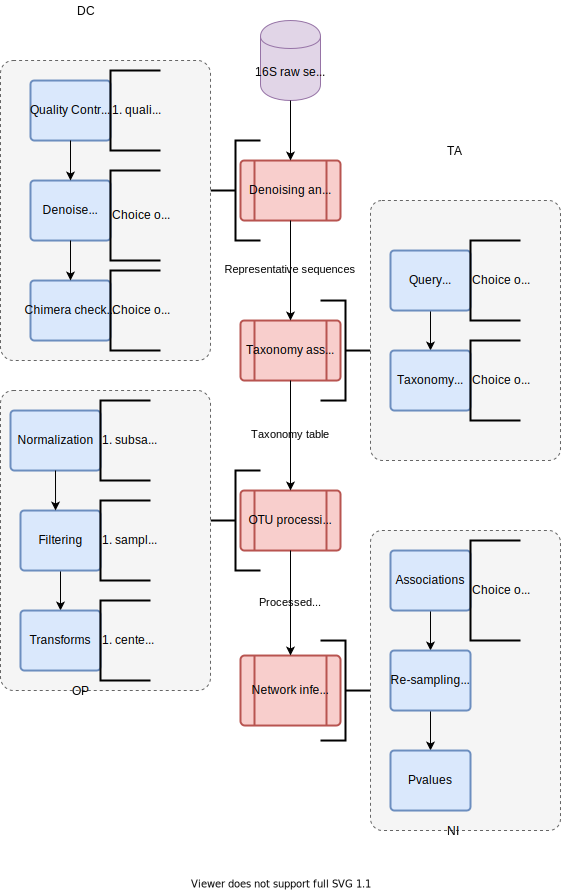
\includegraphics[width=0.74\linewidth]{figure1.pdf}
  % \end{figure}
  \begin{figure}[H]
    \centering
    \caption{
      \textbf{The workflow of the \ac{micone} pipeline}.
      The steps of the workflow can be broken down into five major groups: \textbf{(SP)} \textbf{S}equence \textbf{P}rocessig, \textbf{(DC)} \textbf{D}enoising and \textbf{C}lustering, \textbf{(TA)} \textbf{T}axonomy \textbf{A}ssignment, \textbf{(OP)} \textbf{O}TU and ESV \textbf{P}rocessing, and \textbf{(NI)} \textbf{N}etwork \textbf{I}nference.
      Each step incorporates several processes, each of which in turn have several alternate algorithms for the same task (indicated by the text to the right of the blue boxes).
      The text along the arrows describes the data that is being passed from one step to another.
      The final output of the pipeline is the consensus network generated from the inferred co-occurrence networks.
      For details on each process and the outputs, see Methods.
    }
    \label{fig:figure1}
  \end{figure}



  % \FloatBarrier
  % \newpage
  % \begin{figure}[H]
  %   \centering
  %   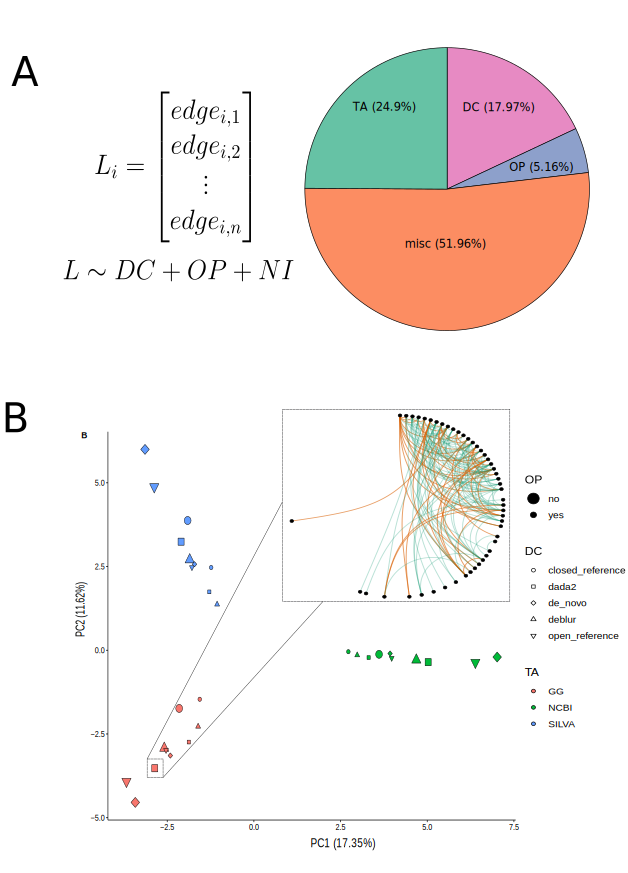
\includegraphics[width=\textwidth]{figure2.pdf}
  % \end{figure}
  \begin{figure}[H]
    \centering
    \caption{
      \textbf{The representative sequences generated by the different DC methods differ in their identification of sequences that are low in abundance.}
      \textbf{(A)} The average weighted UniFrac distance between the representative sequences shows that the representative sequences and their compositions are fairly identical between the methods (with the exception of Deblur (DB)).
      \textbf{(B)} The relatively larger average unweighted UniFrac distance indicates that methods differ in their identification of sequences that are lower in abundance.
      The number of \ac{otu}s or \ac{esv}s generated by the respective methods are provided in the parenthesis next to the names.
      The data used for the analysis in \textbf{(A, B)} were all the samples (healthy and autistic) from the fecal microbiome transplant (FMT) dataset~\cite{Kang2017}.
      \textbf{(C, D)} The distributions of the average weighted and unweighted UniFrac distance between the expected sequence profile and the predicted sequence profile in the mock datasets.
      The distributions of the average weighted UniFrac distance show that de novo (DN) and open reference (OR) were the best-performing methods in most of the datasets, while they are worst performing methods under the unweighted UniFrac metric.
      The good performance of dada2 (D2) under both distance metrics combined with its approach of identifying \ac{esv}s using de novo methods, prompts us to propose it as the default method for the DC step.
      The data used for the analysis in \textbf{(C, D)} were the mock datasets from mockrobiota~\cite{Bokulich2016}.
    }
    \label{fig:figure2}
  \end{figure}


  % \FloatBarrier
  % \newpage
  % \begin{figure}[H]
  %   \centering
  %   \includegraphics[width=\textwidth]{figure3.pdf}
  % \end{figure}
  \begin{figure}[H]
    \centering
    \caption{
      \textbf{Taxonomic reference databases vary in terms of their taxonomy assignments beyond the Order level.}
      \textbf{(A)} The assignments of the top 50 representative sequences to their respective taxonomies using the three different reference databases.
      This result illustrates how the same sequences are assigned to different Genus under different databases.
      A significant portion of the representative sequences are assigned to an ``unknown'' Genus in two of three databases (\ac{gg} and \ac{ncbi}).
      The number of assigned genera for each database are displayed at the top of each column.
      \textbf{(B)} The number of representative sequences assigned to the same taxonomic label when using different reference databases, shown for the top 100 sequences.
      The number of mismatches are fewer at higher taxonomic levels, but, even at the Order level there exists greater than 51\% of mismatches, demonstrating the poor agreement in taxonomic labels assigned by the different databases.
      The data used for the analysis in \textbf{(A, B)} were all the samples (healthy and autistic) from the FMT dataset.
      \textbf{(C)} The Bray-Curtis dissimilarity between the expected taxonomy profile and calculated taxonomy profile in the mock datasets shows that there is no singular best choice of database for every dataset, as all the databases have similar performance.
      The \ac{gg} database and the Naive Bayes classifier are chosen as the defaults for the TA step of \ac{micone}.
      The datasets used for the analysis in \textbf{(C)} were the mock datasets from mockrobiota.
    }
    \label{fig:figure3}
  \end{figure}


  % \FloatBarrier
  % \newpage
  % \begin{figure}[H]
  %   \centering
  %   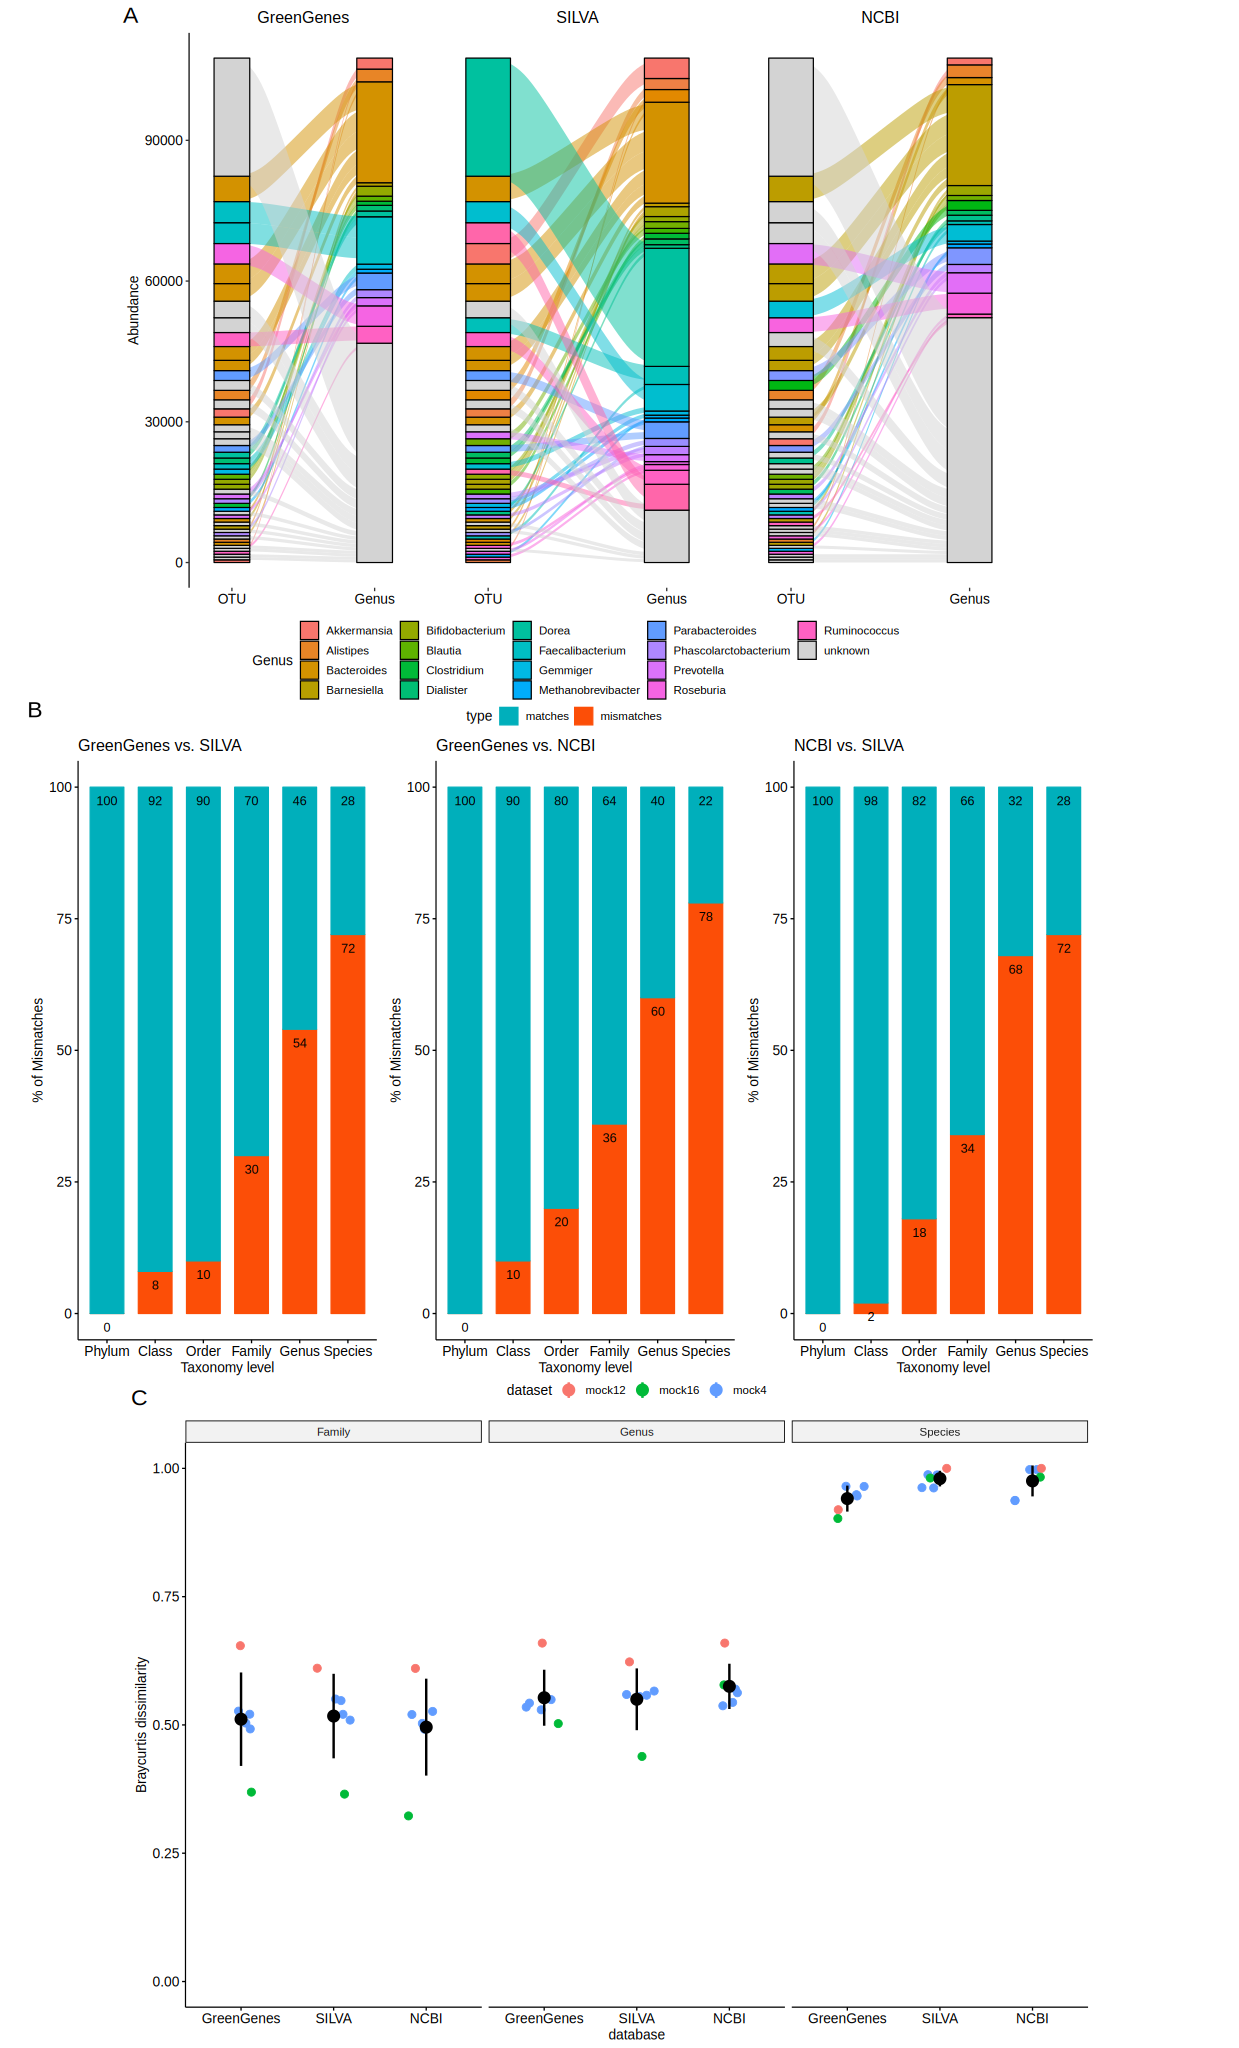
\includegraphics[width=\textwidth]{figure4.pdf}
  % \end{figure}
  \begin{figure}[H]
    \centering
    \caption{
      \textbf{Networks generated using different network inference methods show notable differences both in terms of edge-density and connectivity}.
      \textbf{(A)} The nine different networks (excluding \ac{mldm}) generated by the different network inference methods are very dissimilar.
      The green links are positive associations and the orange links represent negative associations.
      A threshold of 0.3 was set for the correlation-based methods (sparcc, propr, spearman and pearson) and a threshold of 0.01 was set for the direct association methods (flashweave, spieceasi, cozine, harmonies, and spring).
      The correlation-based methods in general produce graph with higher edge-densities.
      \textbf{(B)} The node overlap Upset plot indicates that all the networks have a large proportion of common nodes involved in connections (33 out of 68).
      Whereas, \textbf{(C)} the edge overlap Upset plot shows that a very small fraction of these connections are actually shared (8 out of 202).
      The data used in this analysis were the healthy stool samples from the FMT dataset.
      \ac{mldm} is not shown in the comparisons because the algorithm failed to converge for the particular network combination.
    }
    \label{fig:figure4}
  \end{figure}


  % \FloatBarrier
  % \newpage
  % \begin{figure}[H]
  %   \centering
  %   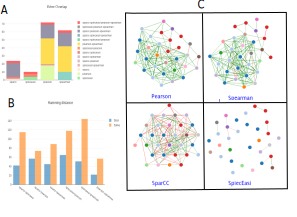
\includegraphics[width=1.0\linewidth]{figure5.pdf}
  % \end{figure}
  \begin{figure}[H]
    \centering
    \caption{
      \textbf{The scaled-sum consensus method returns associations with high precision when applied to the synthetic benchmark datasets}.
      Each point on the box plot shows the precision of the co-occurrence network generated by the individual and consensus methods using the ``NorTA'' and ``seqtime'' methods (refer to Methods).
      The independent algorithms chosen for the comparison are the two best-performing correlation-based (propr, \ac{sparcc}) and direct association based (\ac{spieceasi}, FlashWeave) methods.
      A weight threshold of 0.1 and a p-value threshold of 0.05 was applied to each network before the calculation of precision.
      The different consensus based methods used are the scaled-sum (SS) and simple voting (SV) method.
      The overall best precision was consistently obtained by the scaled-sum method for $p \geq 0.333$ on both datasets.
      Among all the independent network inference methods, \ac{spieceasi} has the best average precision.
      The simple voting method when using presence of edges in all inferred networks as a requirement ($p = 1.000$), also outperforms \ac{spieceasi} on average precision.
      Therefore, we recommend the scaled-sum consensus method with $p = 0.333$ as the default tool for network inference, as this option provides a good balance of precision and sensitivity.
    }
    \label{fig:figure5}
  \end{figure}


  % \FloatBarrier
  % \newpage
  % \begin{figure}[H]
  %   \centering
  %   \includegraphics[width=\textwidth]{figure6.pdf}
  % \end{figure}
  \begin{figure}[H]
    \centering
      \caption{
      \textbf{The choice of reference database contributes has the largest impact on network variance}.
      \textbf{(A)} The percentage of variance in the networks contributed by the DC, CC (chimera checking), TA, OP and NI steps of the pipeline calculated using ANOVA on the linear model, see the Methods section for details.
      The data used for the analysis were the healthy stool samples from the FMT dataset.
      A weight threshold of 0.1 and a p-value threshold of 0.05 was applied to each network before the analysis.
      The taxonomy database contributes most to the variance between the networks (65.4\%) followed by the filtering of the counts matrix (26.8\%) in the OP step.
    The variation due to the DC and CC steps are much smaller in comparison (0.648\% and 0.003\% respectively).
      The fraction labeled as the residual is an artifact that arises when multiple steps are changed at the same time, however, this can be ignored as this fraction is negligible.
      \textbf{(B)} All combinations of inferred networks are shown as points on a PCA plot.
      Each point on the PCA plot represents a network inferred using different combinations of tools and parameters that are available in the \ac{micone} pipeline.
      The color of the points corresponds to the tools used at each step of the pipeline (DC, TA, OP and NI).
      The points on the PCA plot can be grouped based on the TA step, but at the NI step only some methods create high variability in the inferred networks.
      The \ac{dc} step does not seem to have any correlation with the similarity of networks on the PCA plot, but all the networks with filtering at the \ac{op} step are similar to each other.
      This further confirms that the variability in the networks decreases upon filtering out the taxonomic entities at low abundance.
    }
    \label{fig:figure6}
  \end{figure}


  % \FloatBarrier
  % \newpage
  % \begin{figure}[H]
  %   \centering
  %   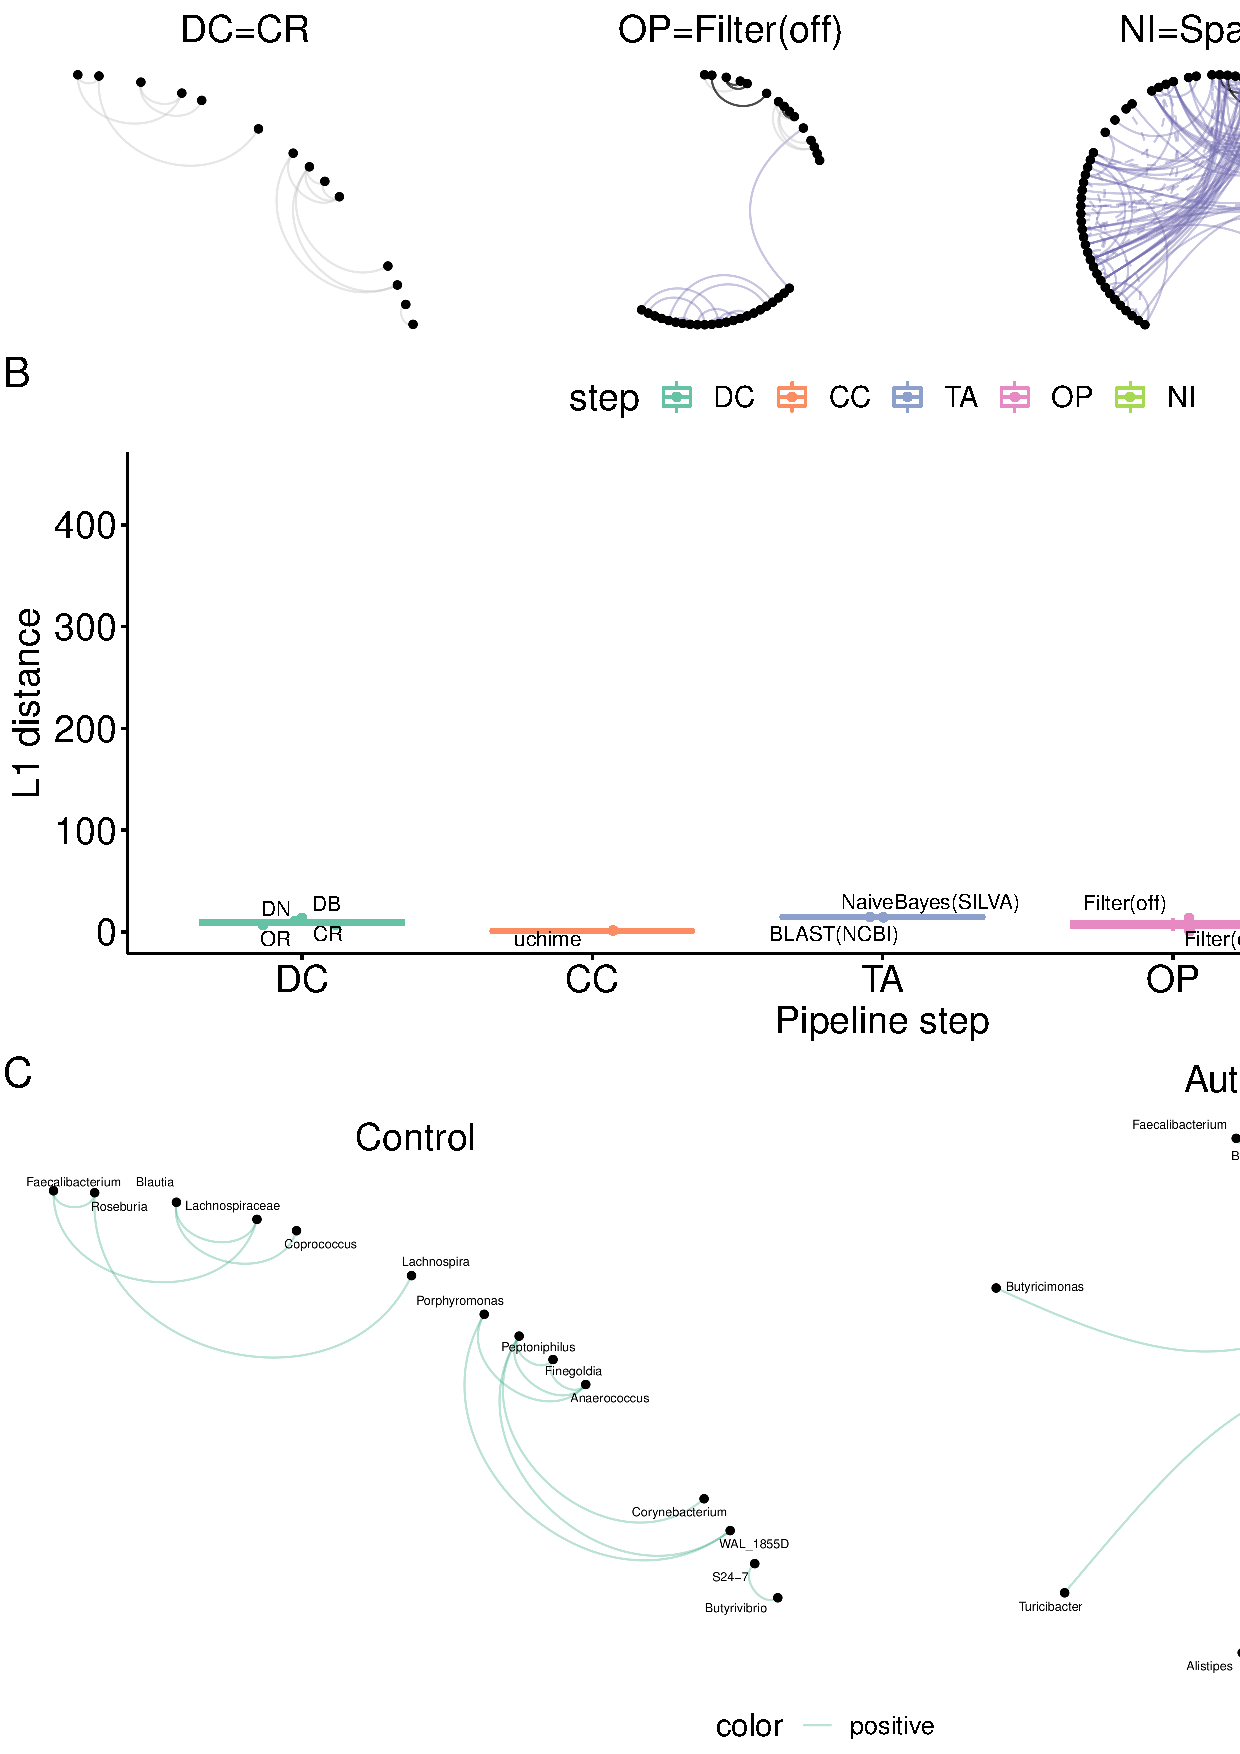
\includegraphics[width=1.0\linewidth]{figure7.pdf}
  % \end{figure}
  \begin{figure}[H]
    \centering
    \caption{
      \textbf{Comparison of networks generated from autistic and control samples using the \ac{micone} pipeline}.
      The networks for the control (left) and autistic (right) samples in the FMT dataset were generated using the default tools and parameters recommended by the \ac{micone} pipeline.
      There are 20 unique links in the network for control samples, 12 unique links in the network for autistic subjects and 7 edges in common between both networks.
    }
    \label{fig:figure7}
  \end{figure}


  \subsection*{Supplementary figures}

    % \begin{figure}[H]
    %   \centering
    %   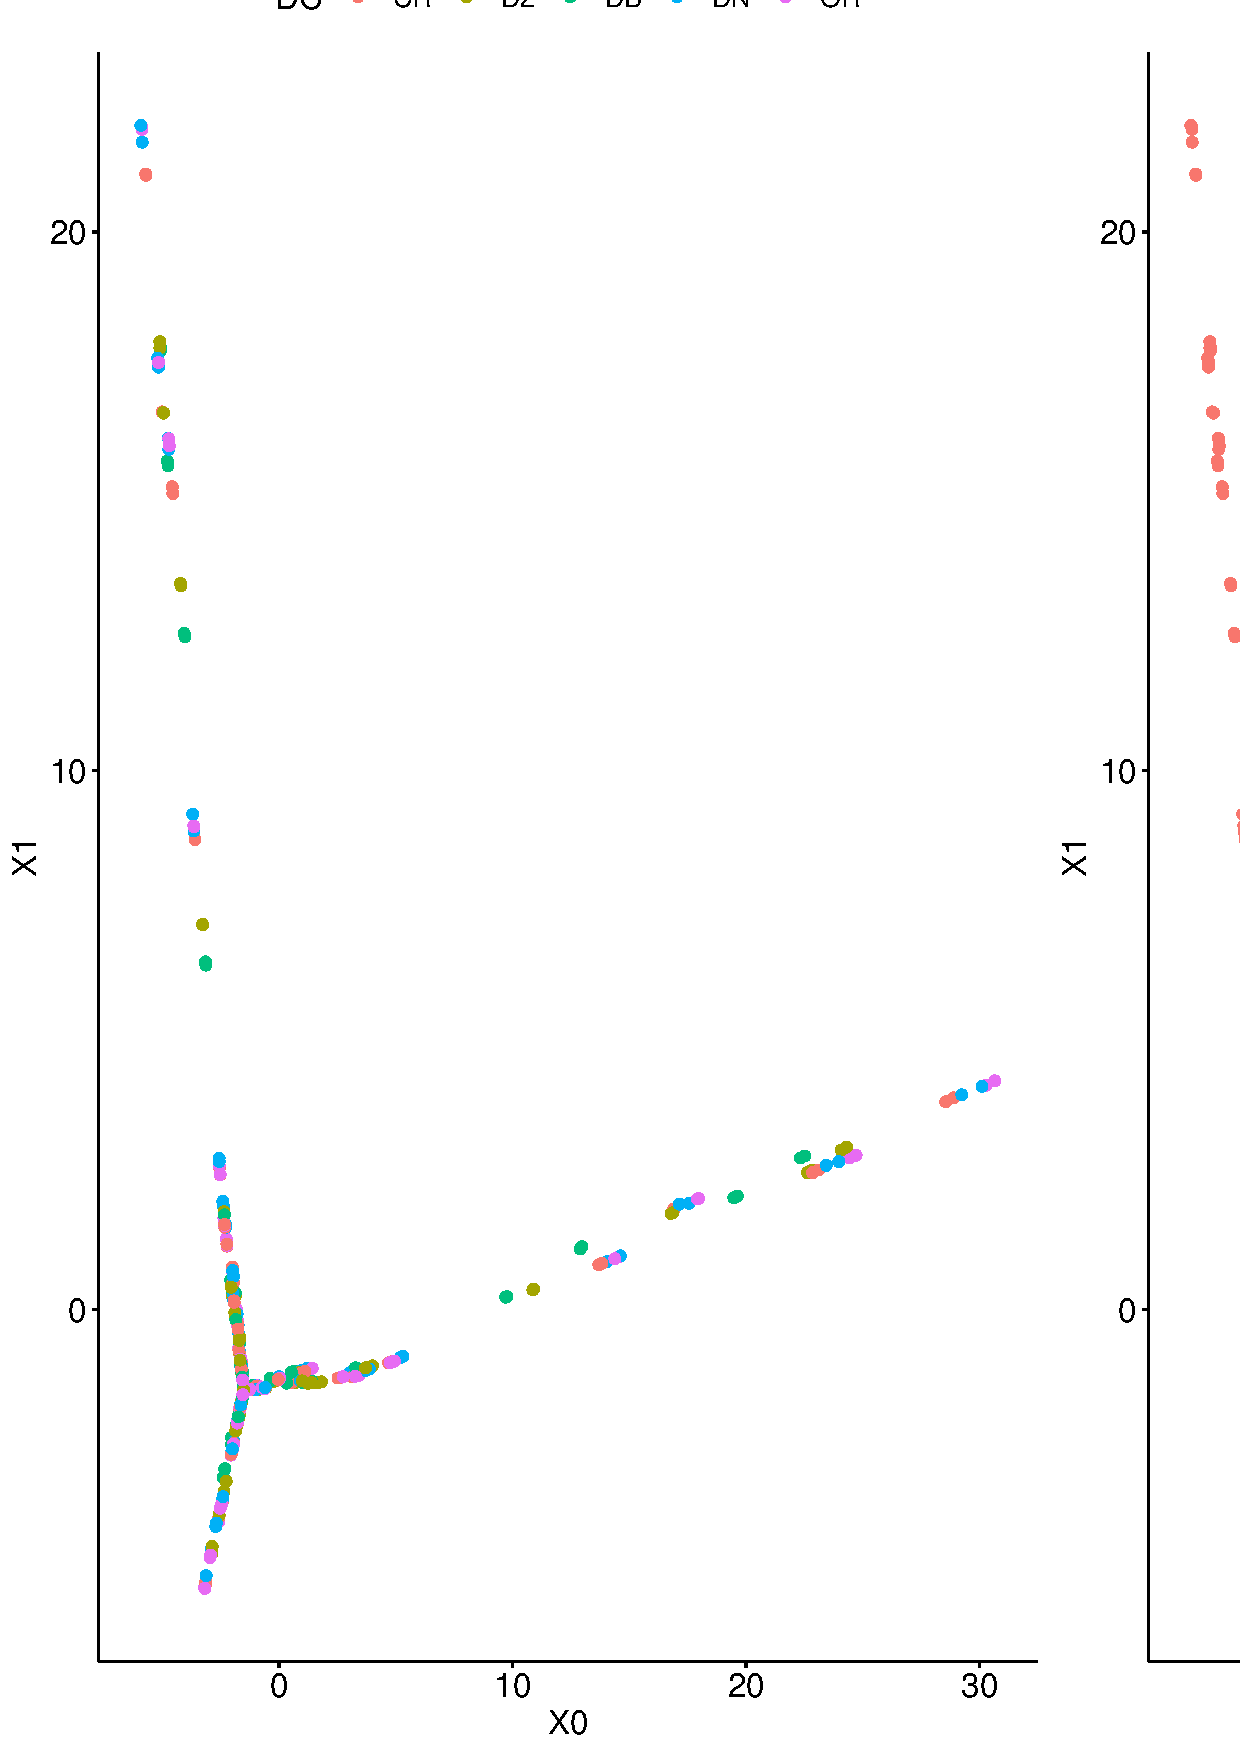
\includegraphics[width=1.0\linewidth]{figure_s1.pdf}
    % \end{figure}
    \begin{figure}[H]
      \centering
        \caption{
          \textbf{The t-SNE plot of all the inferred networks clusters the networks based on the taxonomy reference database used}.
          Each point on the t-SNE plot represents a network inferred using different combinations of tools and parameters that are available in the \ac{micone} pipeline.
          The points are colored by the tools and parameters used in \ac{dc} step (A), \ac{ta} step (B), \ac{op} step (C) and \ac{ni} step (D).
          The separation of the points based on taxonomy reference database shows that the points cluster based on reference database in high-dimensional space.
        }
      \label{fig:figure_s1}
    \end{figure}
    % \FloatBarrier
    % \newpage

    % \begin{figure}[H]
    %   \centering
    %   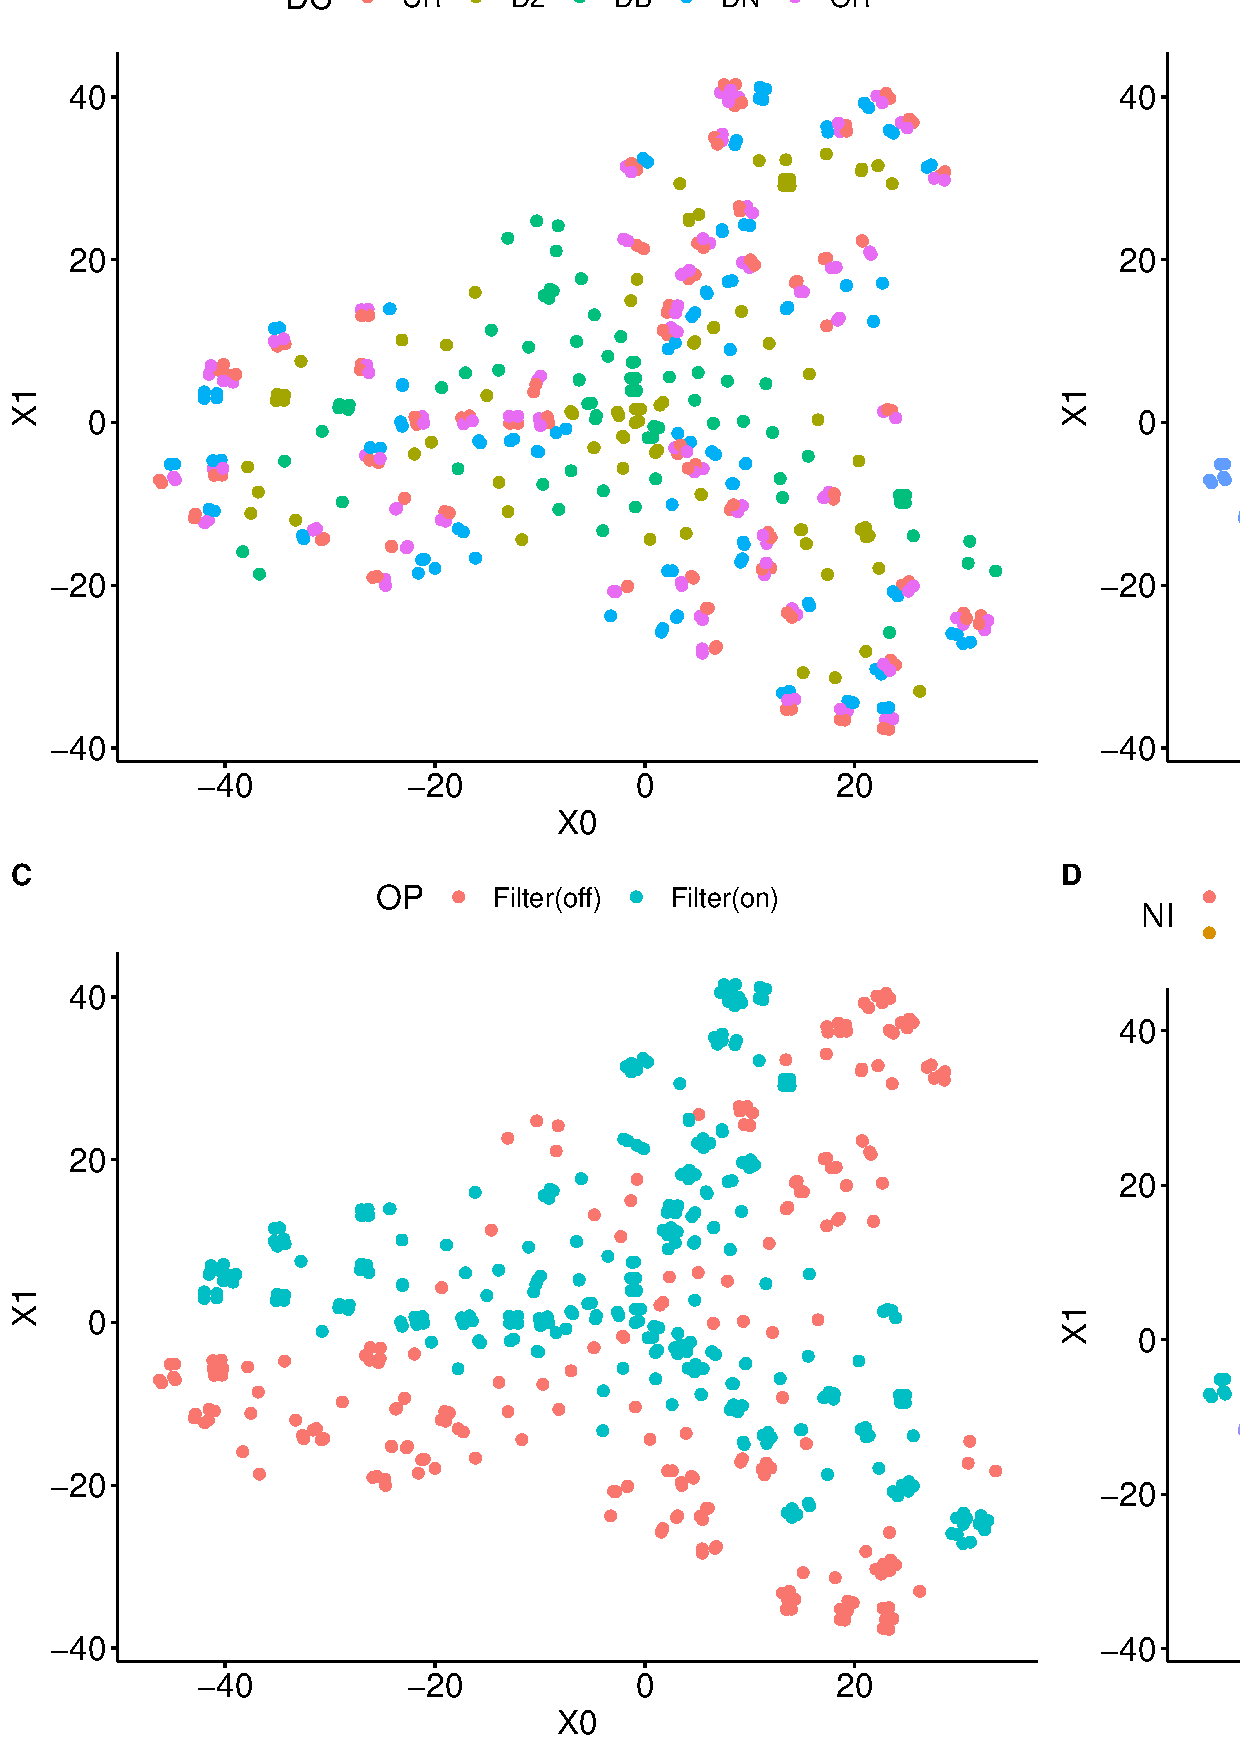
\includegraphics[width=1.0\linewidth]{figure_s2.pdf}
    % \end{figure}
    \begin{figure}[H]
      \centering
        \caption{
          \textbf{The UniFrac distance between the 1000 most abundant representative sequences is higher than that when all sequences are considered}.
          Each value is the average UniFrac distance between the reference sequences generated by the various methods in the \ac{dc} step (similar to Figure~\ref{fig:figure2}).
          There is an increase in both weighted and unweighted UniFrac distances compared to when all the representative sequences are considered.
          This shows that the 1000 most abundant representative sequences generated by the methods are not as similar to each other.
          And since the weighted UniFrac is much smaller than the unweighted UniFrac distance, we can conclude that those reference sequences that are present in the middle of the abundance distribution are dissimilar.
        }
      \label{fig:figure_s2}
    \end{figure}
    % \FloatBarrier
    % \newpage

    % \begin{figure}[H]
    %   \centering
    %   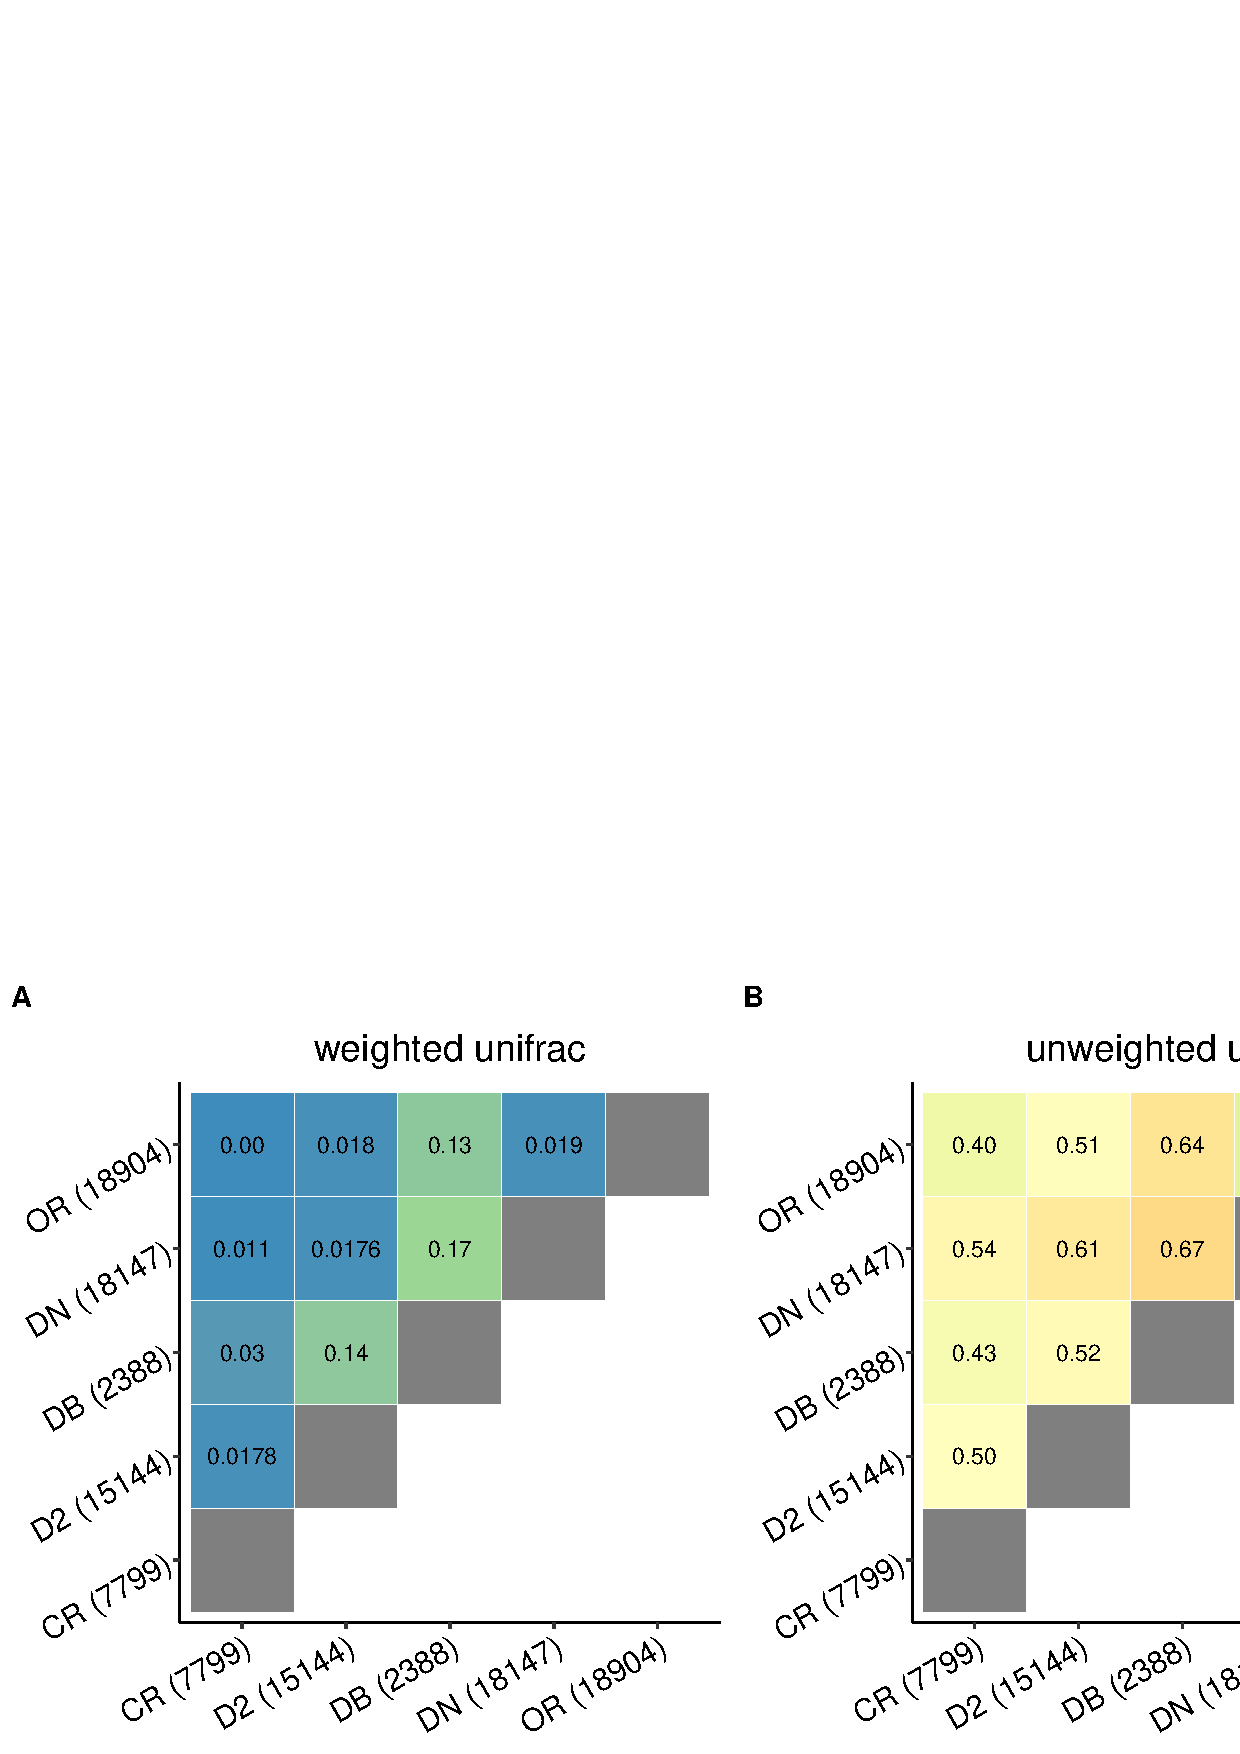
\includegraphics[width=1.0\linewidth]{figure_s3.pdf}
    % \end{figure}
    \begin{figure}[H]
      \centering
        \caption{
          \textbf{The weighted and unweighted UniFrac distances between representative sequences generated using remove bimera and uchime for each denoising method are low.}
          The two chimera checking methods, uchime and remove bimera, produce similar outputs.
          With the exception of de novo and open reference under the unweighted UniFrac metric, all the other methods have low dissimilarity.
          This is especially true for the \ac{dada2} and Deblur methods which are the recommended denoising methods in the \ac{micone} pipeline.
          Therefore, remove bimera is recommended as the default chimera method if one is using \ac{dada2} and uchime-denovo when one is using Deblur, since these methods were developed for these respective algorithms (\ac{qiime2} uses uchime-denovo in the Deblur workflow).
        }
      \label{fig:figure_s3}
    \end{figure}
    % \FloatBarrier
    % \newpage

    % \begin{figure}[H]
    %   \centering
    %   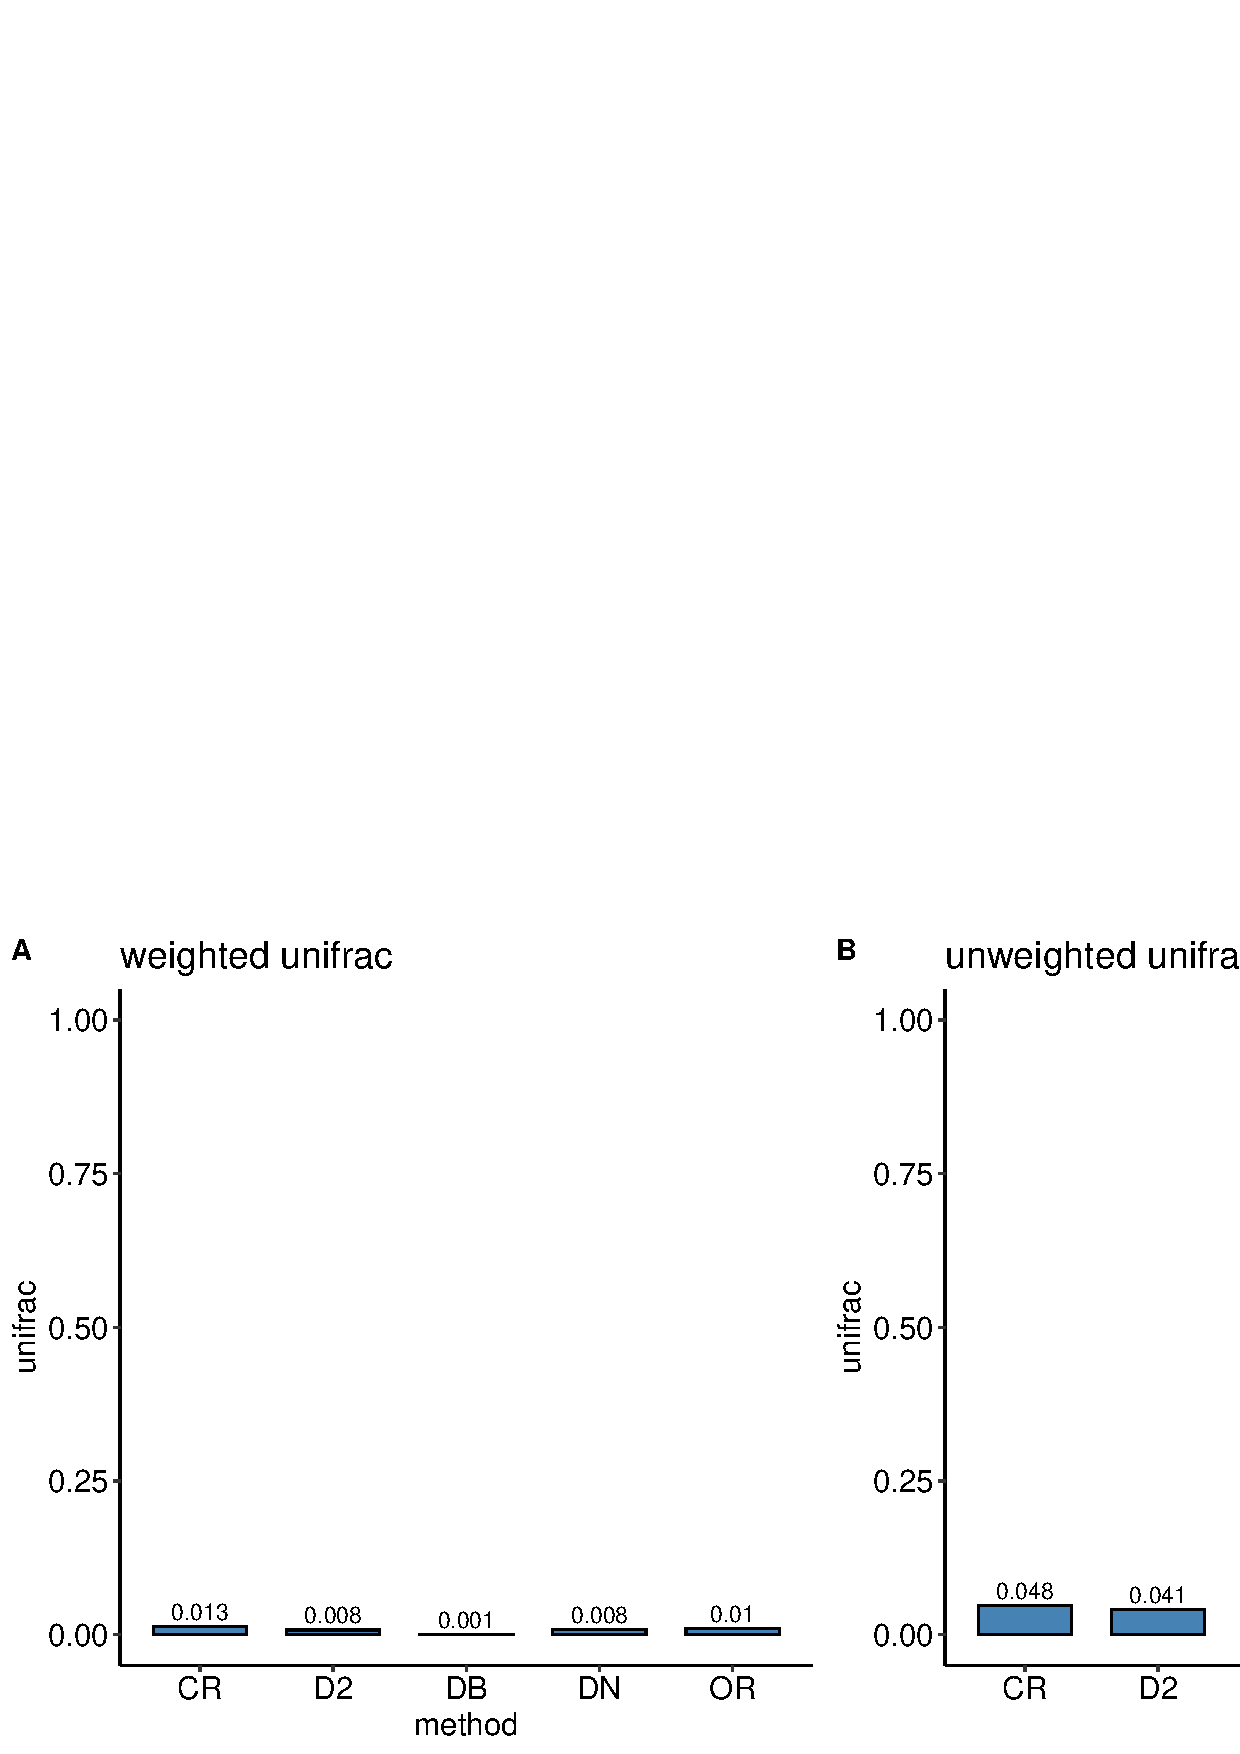
\includegraphics[width=1.0\linewidth]{figure_s4.pdf}
    % \end{figure}
    \begin{figure}[H]
      \centering
        \caption{
          \textbf{The pairwise comparison of assignments generated using different databases for all representative sequences has a higher proportion of mismatches}.
          The comparison made here is similar to Figure~\ref{fig:figure3}B, but instead of the top 100 taxonomic entities (by abundance), all the assignments from one database are matched with those from the other two databases.
          Higher percentage of mismatches implies that the matching of the taxonomies in the more abundant sequences (top 100) are more consistent.
        }
      \label{fig:figure_s4}
    \end{figure}
    % \FloatBarrier
    % \newpage

  % \begin{figure}[H]
  %   \centering
  %   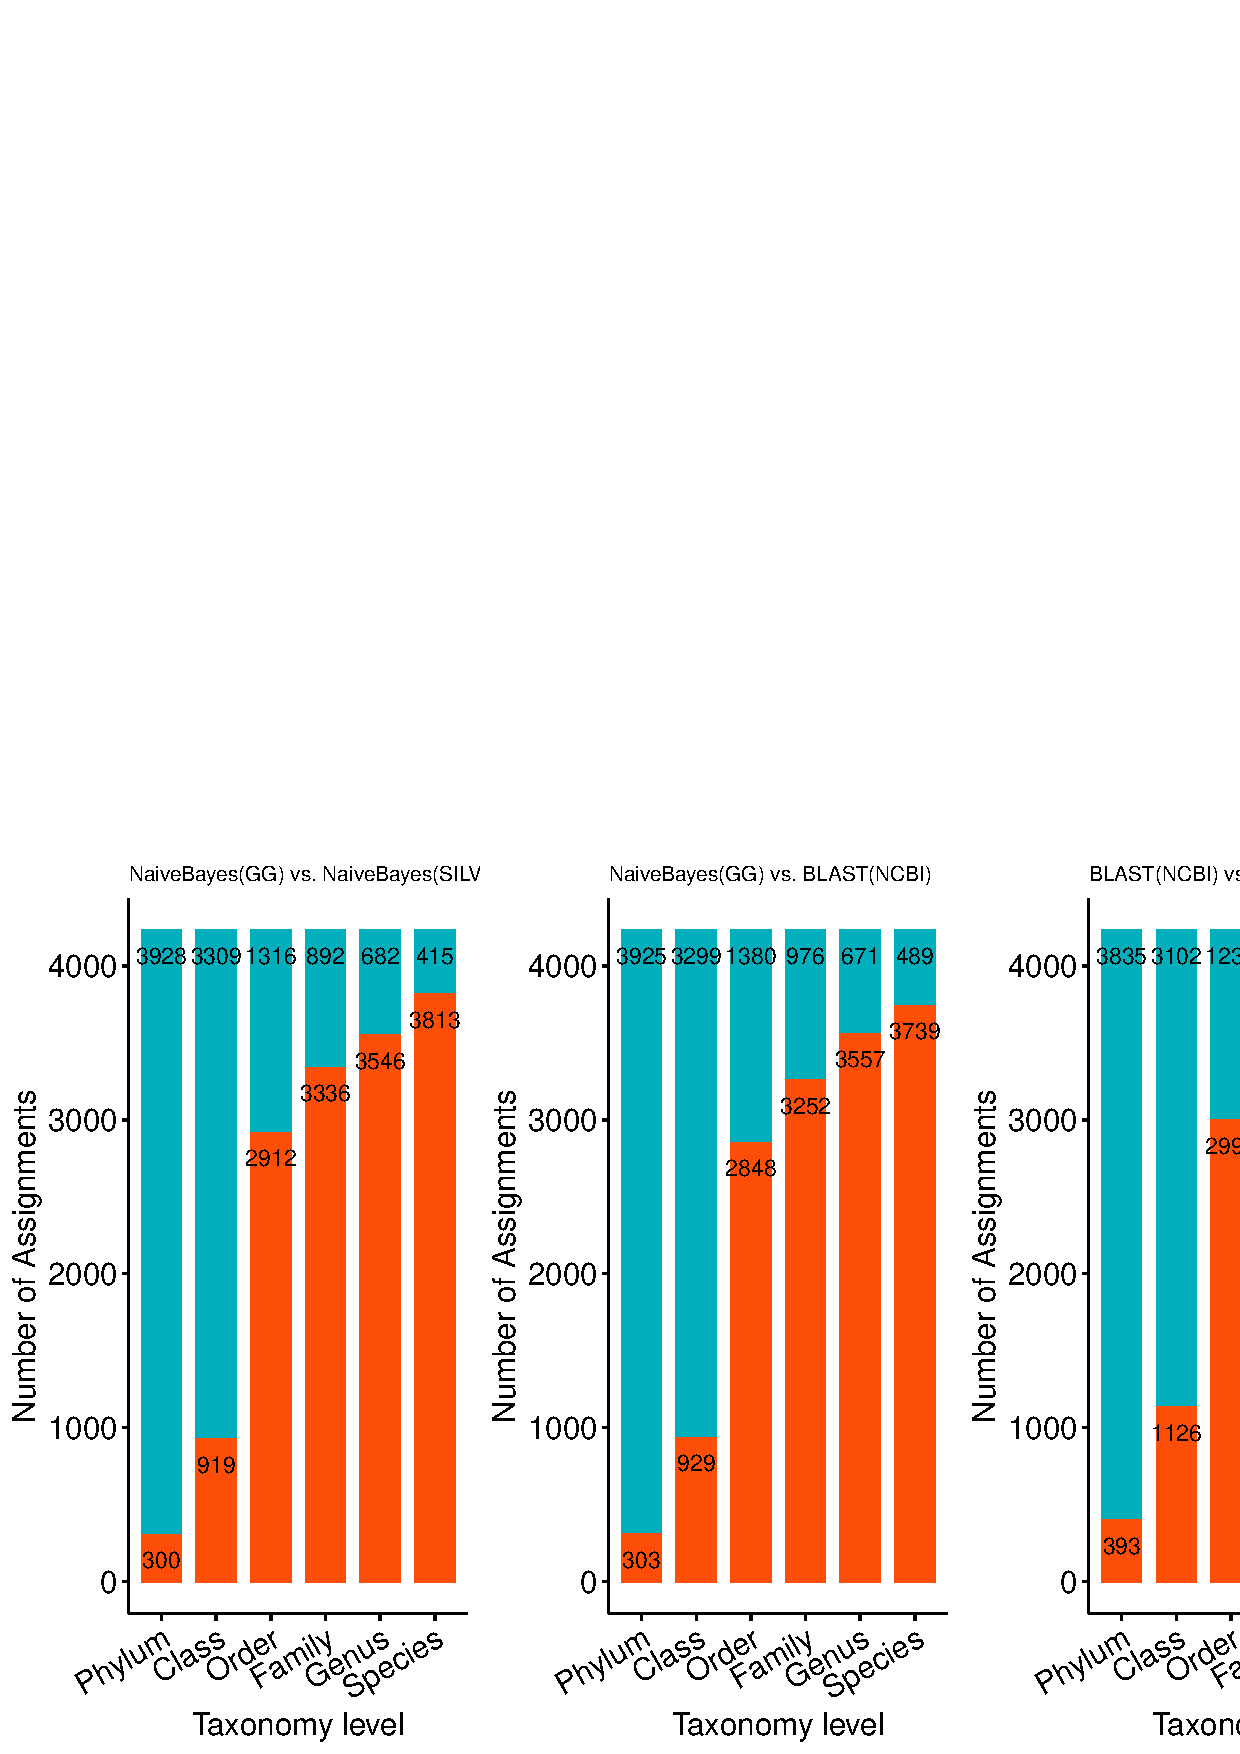
\includegraphics[width=1.0\linewidth]{figure_s5.pdf}
  % \end{figure}
  \begin{figure}[H]
    \centering
      \caption{
        \textbf{The precision and sensitivity of the inferred networks on the ``NorTA'' synthetic interaction data.}
        The different consensus based methods used are: scaled-sum (SS) and simple voting (SV) method.
        Pearson and Spearman methods are not used in the calculation of the consensus.
        Among all the independent network inference methods, \ac{spieceasi} has the best average precision (0.944), but the overall best precision was consistently obtained by the scaled-sum method (0.956, 0.985 and 1.000).
        The simple voting method when using presence of edges in all inferred networks as a requirement ($p = 1.000$), also outperforms \ac{spieceasi} on average precision (0.969).
        Although \ac{spieceasi} has a higher performance on sensitivity, if the goal of network inference is to obtain the list of associations that have a high probability of existing in the real microbial community, then the consensus methods perform better.
      }
    \label{fig:figure_s5}
  \end{figure}
  % \FloatBarrier
  % \newpage

  % \begin{figure}[H]
  %   \centering
  %   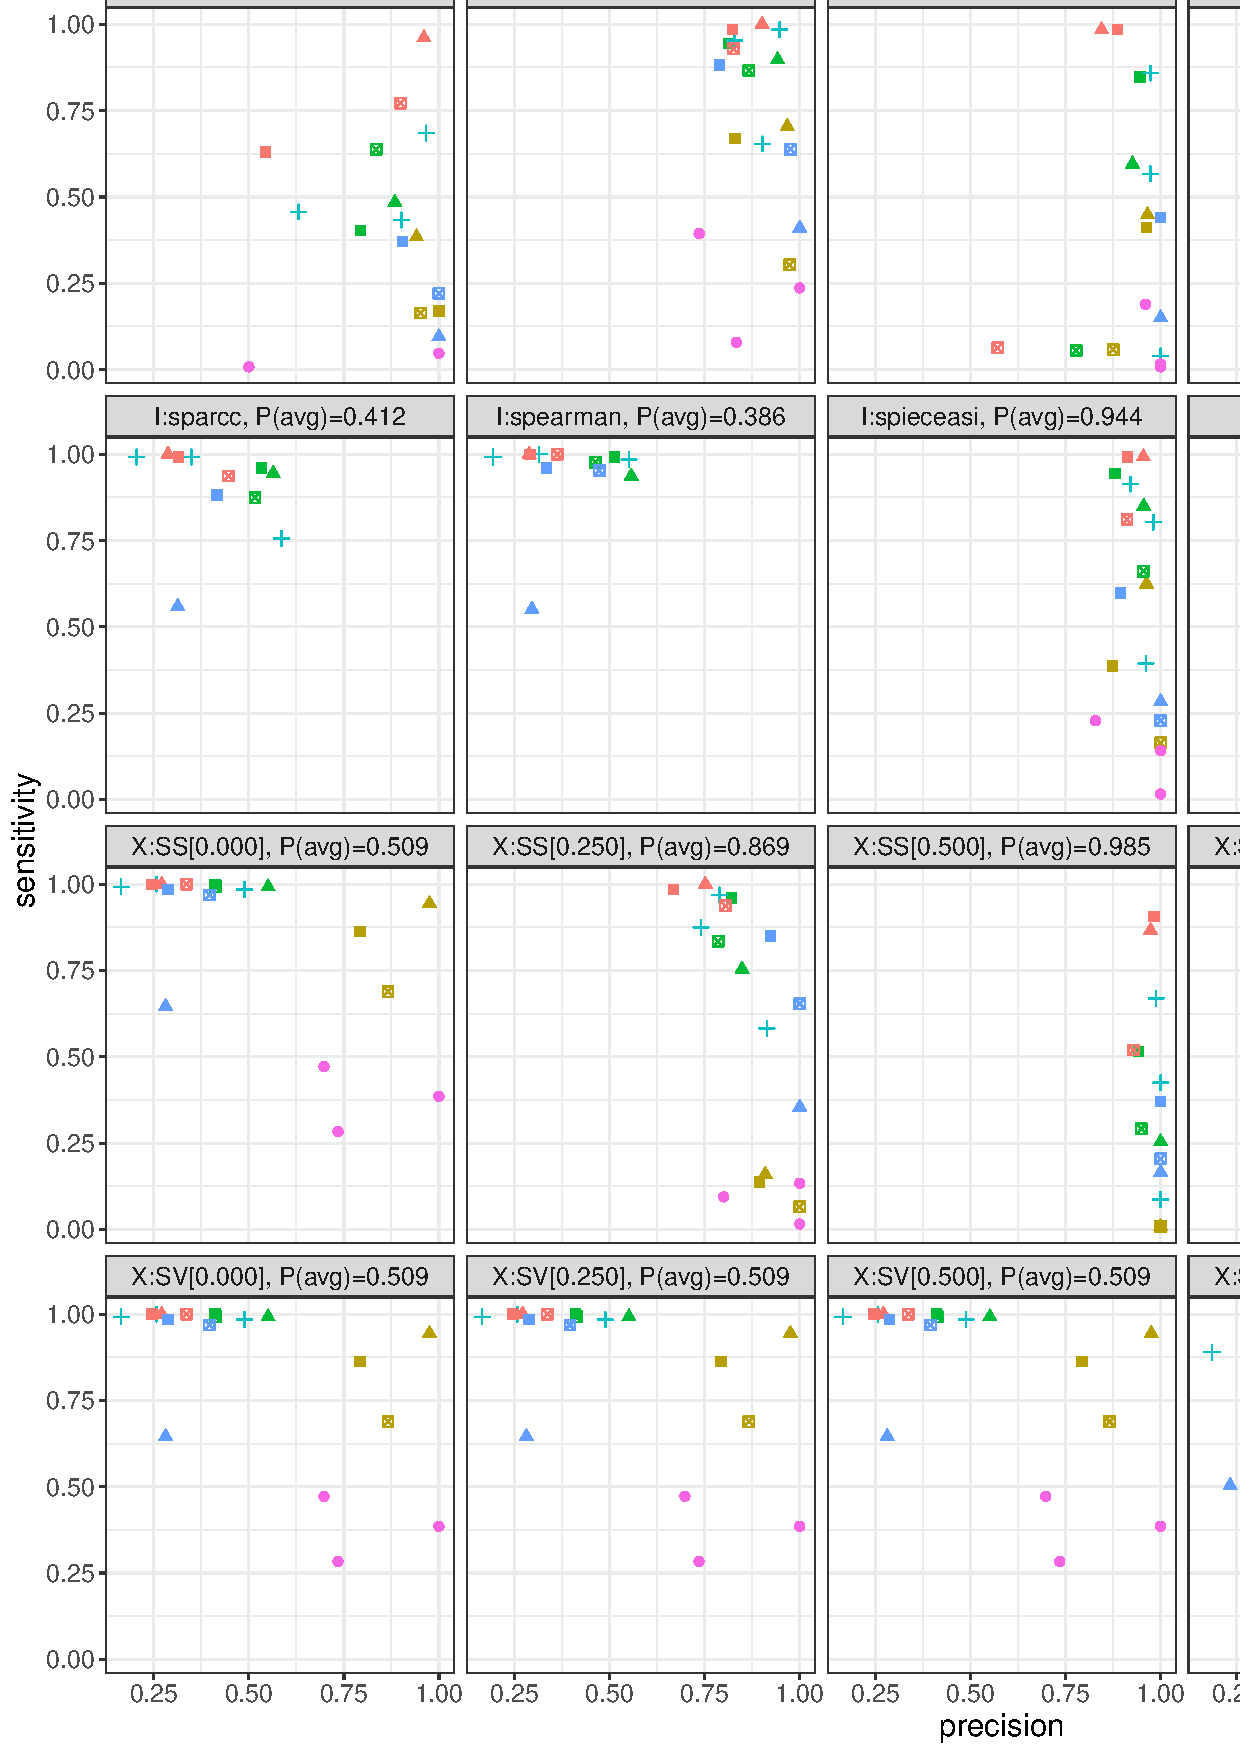
\includegraphics[width=1.0\linewidth]{figure_s6.pdf}
  % \end{figure}
  \begin{figure}[H]
    \centering
      \caption{
        \textbf{The precision and sensitivity of the inferred networks on the ``seqtime'' synthetic interaction data.}
        The different consensus based methods used are: scaled-sum (SS) and simple voting (SV) method.
        Pearson and Spearman methods are not used in the calculation of the consensus.
        Among all the independent network inference methods, \ac{spieceasi} has the best average precision (0.624), but the overall best precision was consistently obtained by the scaled-sum method (0.688, 0.820 and 1.000).
        The simple voting method when using presence of edges in all inferred networks as a requirement ($p = 1.000$), also outperforms \ac{spieceasi} on average precision (0.692).
        These results show that the scaled-sum method is not only much better suited for inferring robust and accurate interactions from count data regardless of the distributions and topologies, but it is also capable of accurately extracting real associations (gLV interactions) from count data.
      }
    \label{fig:figure_s6}
  \end{figure}
  % \FloatBarrier
  % \newpage

  % \begin{figure}[H]
  %   \centering
  %   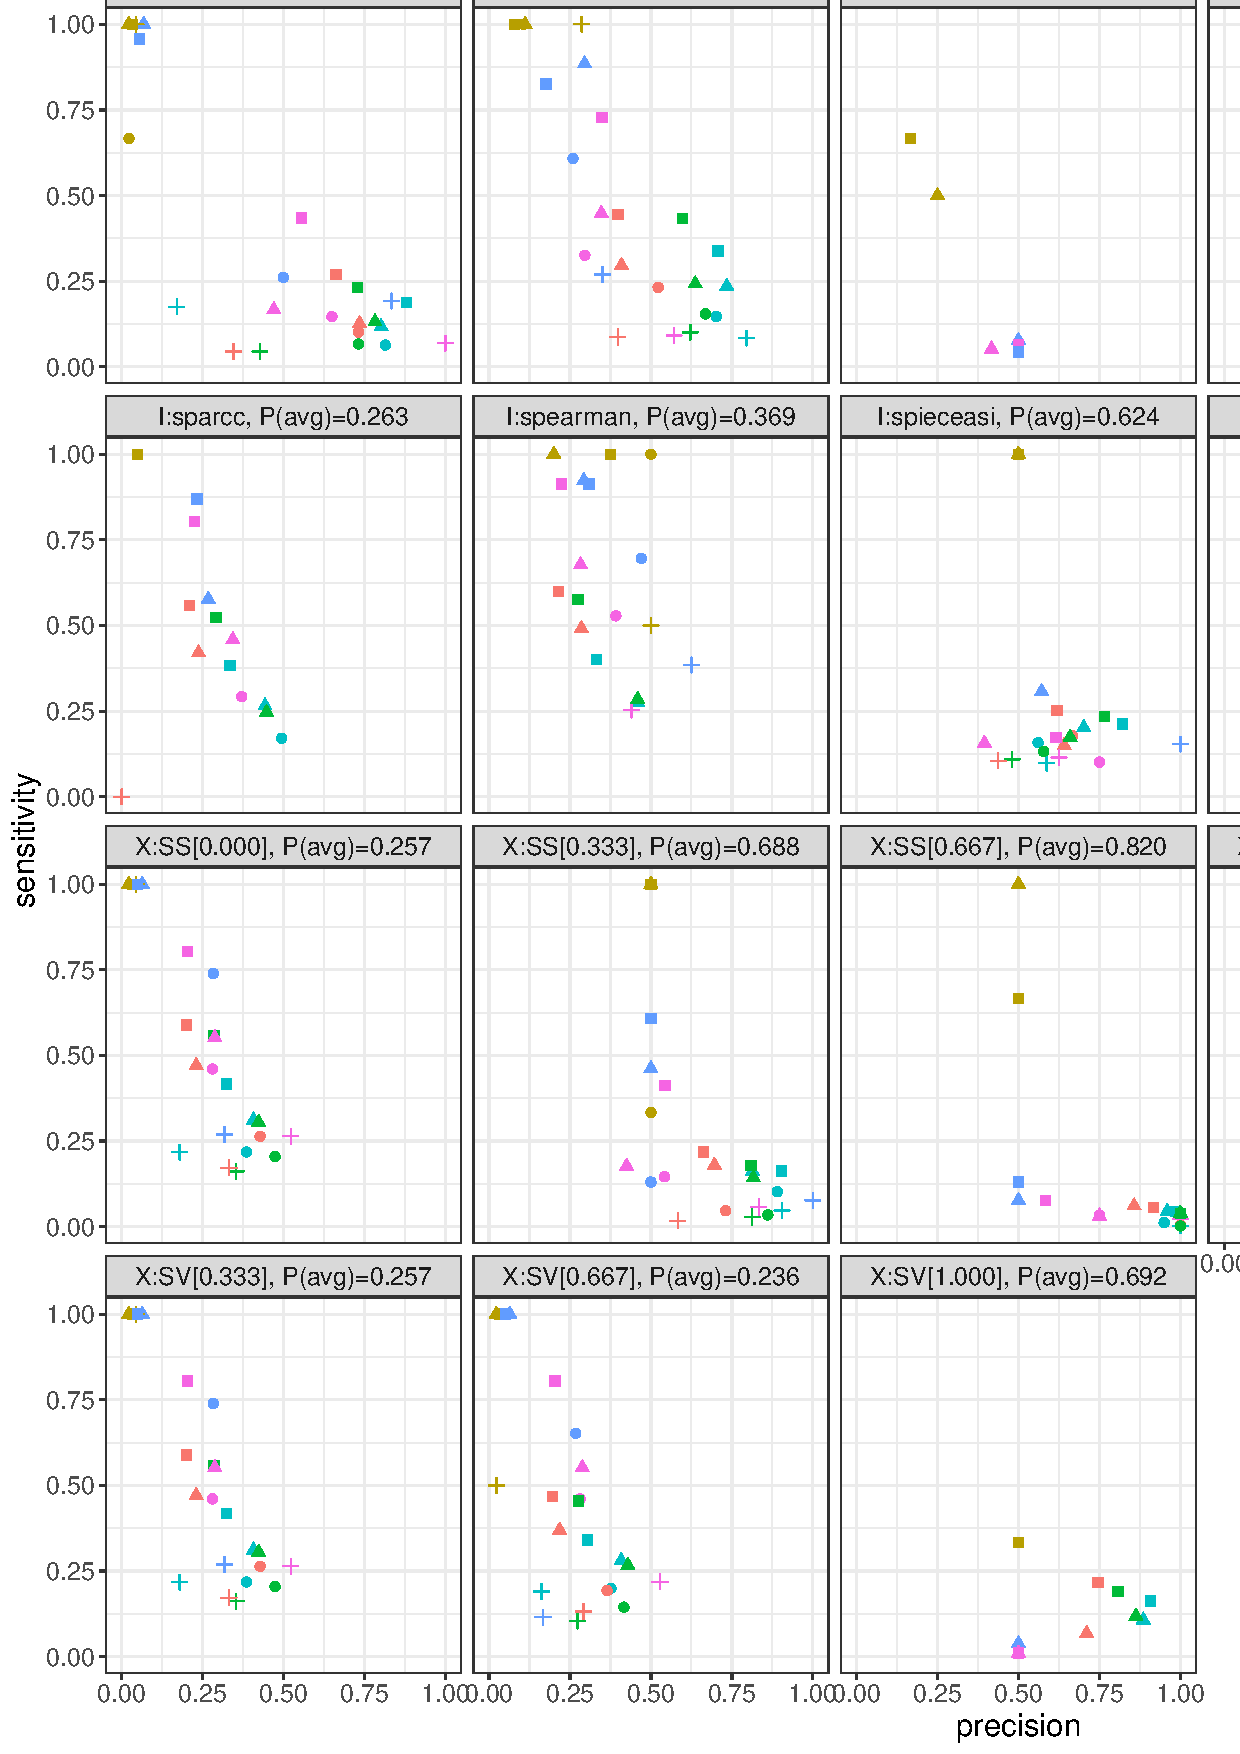
\includegraphics[width=1.0\linewidth]{figure_s7.pdf}
  % \end{figure}
  \begin{figure}[H]
    \centering
    \caption{
      \textbf{Sensitivity analysis of the default settings of the \ac{micone} pipeline}.
      \textbf{(A)} The network constructed using the default pipeline parameters (DC=\ac{dada2}, CC=remove bimera, TA=\ac{gg}, OP=Filter(on), NI=scaled-sum consensus) is compared with networks generated when one of the steps use a different tool.
      The layout is created by fixing the positions of all the nodes from all networks and then drawing only the relevant edges.
      The edges colored green are positive associations and those in red are negative associations.
      We observe that changing the TA and OP steps leads to the creation of the most number of unique edges.
      \textbf{(B)} The dot plot showing the fraction of nodes (left) and edges (right) in common between the default network and the networks generated by changing one step of the default pipeline.
      The low value of the common fraction for TA and OP steps shows that these steps induce the biggest changes nodes and edges.
      The NI step is not shown in this analysis because the consensus method uses edges from the individual network inference methods and a comparison would be biased.
    }
    \label{fig:figure_s7}
  \end{figure}
  % \FloatBarrier
  % \newpage


%!TEX root = ../main.tex

\newpage
\section*{Supplementary}

  \renewcommand{\thefigure}{S\arabic{figure}}
  \setcounter{figure}{0}

  \renewcommand{\thetable}{S\arabic{table}}
  \setcounter{table}{0}

  \begin{table}[h]
\resizebox{\textwidth}{!}{
\begin{tabular}{lllll}
\hline
\textbf{Step}                             & \textbf{Task}                                            & \textbf{Tool}                          & \textbf{Parameter}                     & \textbf{Value}                                                                                           \\ \hline
\multirow{29}{*}{Denosing and Clustering} & \multicolumn{1}{c}{\multirow{9}{*}{Sequence Processing}} & \multirow{2}{*}{join\_reads}           & min\_overlap                           & 6                                                                                                        \\
                                          & \multicolumn{1}{c}{}                                     &                                        & perc\_max\_diff                        & 8                                                                                                        \\
                                          & \multicolumn{1}{c}{}                                     & \multirow{2}{*}{demultiplex\_illumina} & rev\_comp\_barcodes                    & False                                                                                                    \\
                                          & \multicolumn{1}{c}{}                                     &                                        & rev\_comp\_mapping\_barcodes           & False                                                                                                    \\
                                          & \multicolumn{1}{c}{}                                     & demultiplex\_454                       & -                                      & -                                                                                                        \\
                                          & \multicolumn{1}{c}{}                                     & \multirow{4}{*}{trim\_filter\_fixed}   & seq\_sample\_size                      & 10,000                                                                                                   \\
                                          & \multicolumn{1}{c}{}                                     &                                        & ncpus                                  & 1                                                                                                        \\
                                          & \multicolumn{1}{c}{}                                     &                                        & trunc\_q                               & 2                                                                                                        \\
                                          & \multicolumn{1}{c}{}                                     &                                        & max\_ee                                & 2                                                                                                        \\ \cline{2-5}
                                          & \multirow{3}{*}{Chimera Checking}                        & uchime                                 & -                                      & -                                                                                                        \\
                                          &                                                          & \multirow{2}{*}{remove\_bimera}        & ncpus                                  & 1                                                                                                        \\
                                          &                                                          &                                        & chimera\_method                        & consensus                                                                                                \\ \cline{2-5}
                                          & \multirow{17}{*}{Denoise Cluster}                        & \multirow{3}{*}{de\_novo}              & enable\_rev\_strand\_match             & True                                                                                                     \\
                                          &                                                          &                                        & suppress\_de\_novo\_chimera\_detection & True                                                                                                     \\
                                          &                                                          &                                        & ncpus                                  & 1                                                                                                        \\
                                          &                                                          & \multirow{4}{*}{closed\_reference}     & enable\_rev\_strand\_match             & True                                                                                                     \\
                                          &                                                          &                                        & suppress\_de\_novo\_chimera\_detection & True                                                                                                     \\
                                          &                                                          &                                        & ncpus                                  & 1                                                                                                        \\
                                          &                                                          &                                        & reference\_sequences                   & 97\_otus.fasta                                                                                           \\
                                          &                                                          & \multirow{5}{*}{open\_reference}       & enable\_rev\_strand\_match             & True                                                                                                     \\
                                          &                                                          &                                        & suppress\_de\_novo\_chimera\_detection & True                                                                                                     \\
                                          &                                                          &                                        & ncpus                                  & 1                                                                                                        \\
                                          &                                                          &                                        & reference\_sequences                   & 97\_otus.fasta                                                                                           \\
                                          &                                                          &                                        & picking\_method                        & uclust                                                                                                   \\
                                          &                                                          & \multirow{2}{*}{dada2}                 & ncpus                                  & 1                                                                                                        \\
                                          &                                                          &                                        & big\_data                              & FALSE                                                                                                    \\
                                          &                                                          & \multirow{3}{*}{deblur}                & ncpus                                  & 1                                                                                                        \\
                                          &                                                          &                                        & mind\_reads                            & 2                                                                                                        \\
                                          &                                                          &                                        & min\_size                              & 2                                                                                                        \\ \hline
\multirow{7}{*}{Taxonomy Assignment}      & \multirow{7}{*}{Assign}                                  & \multirow{3}{*}{naive\_bayes}          & confidence                             & 0.7                                                                                                      \\
                                          &                                                          &                                        & mem\_per\_core                         & 8G                                                                                                       \\
                                          &                                                          &                                        & ncpus                                  & 1                                                                                                        \\
                                          &                                                          & \multirow{4}{*}{blast}                 & max\_accepts                           & 10                                                                                                       \\
                                          &                                                          &                                        & perc\_identity                         & 0.8                                                                                                      \\
                                          &                                                          &                                        & evalue                                 & 0.001                                                                                                    \\
                                          &                                                          &                                        & min\_consensus                         & 0.51                                                                                                     \\ \hline
\multirow{12}{*}{OTU/ESV Processing}      & \multirow{5}{*}{Filter}                                  & \multirow{3}{*}{abundance}             & count\_thres                           & 500                                                                                                      \\
                                          &                                                          &                                        & prevalence\_thres                      & 0.05                                                                                                     \\
                                          &                                                          &                                        & abundance\_thres                       & 0.01                                                                                                     \\
                                          &                                                          & group                                  & tax\_levels                            & \begin{tabular}[c]{@{}l@{}}{[}'Phylum', 'Class', 'Order',\\ 'Family', 'Genus', 'Species'{]}\end{tabular} \\
                                          &                                                          & partition                              & -                                      & -                                                                                                        \\ \cline{2-5}
                                          & \multirow{6}{*}{Transform}                               & \multirow{6}{*}{normalize}             & count\_thres                           & 500                                                                                                      \\
                                          &                                                          &                                        & axis                                   & sample                                                                                                   \\
                                          &                                                          &                                        & prevalence\_thres                      & 0.05                                                                                                     \\
                                          &                                                          &                                        & abundace\_thres                        & 0.01                                                                                                     \\
                                          &                                                          &                                        & rm\_sparse\_obs                        & True                                                                                                     \\
                                          &                                                          &                                        & rm\_sparse\_samples                    & True                                                                                                     \\ \cline{2-5}
                                          & Export                                                   & biom2tsv                               & -                                      & -                                                                                                        \\ \hline
\multirow{17}{*}{Network Inference}       & \multirow{4}{*}{Bootstrap}                               & \multirow{3}{*}{resample}              & bootstraps                             & 1000                                                                                                     \\
                                          &                                                          &                                        & ncpus                                  & 1                                                                                                        \\
                                          &                                                          &                                        & filter\_flag                           & True                                                                                                     \\
                                          &                                                          & pvalue                                 & ncpus                                  & 1                                                                                                        \\ \cline{2-5}
                                          & \multirow{12}{*}{Correlation}                            & \multirow{2}{*}{sparcc}                & iterations                             & 50                                                                                                       \\
                                          &                                                          &                                        & ncpus                                  & 1                                                                                                        \\
                                          &                                                          & pearson                                & -                                      & -                                                                                                        \\
                                          &                                                          & spearman                               & -                                      & -                                                                                                        \\
                                          &                                                          & \multirow{5}{*}{spieceasi}             & method                                 & mb                                                                                                       \\
                                          &                                                          &                                        & ncpus                                  & 1                                                                                                        \\
                                          &                                                          &                                        & nreps                                  & 50                                                                                                       \\
                                          &                                                          &                                        & nlambda                                & 20                                                                                                       \\
                                          &                                                          &                                        & lambda\_min\_ratio                     & 1e-2                                                                                                     \\
                                          &                                                          & \multirow{2}{*}{mldm}                  & z\_mean                                & 1                                                                                                        \\
                                          &                                                          &                                        & max\_iteration                         & 1500                                                                                                     \\
                                          &                                                          & magma                                  & -                                      & -                                                                                                        \\ \cline{2-5}
                                          & Network                                                  & make\_network                          & -                                      & -                                                                                                        \\ \hline
\end{tabular}
}
\caption{The default parameters used in the various tools of the pipeline}
\label{tab:all_parameters}
\end{table}


  \subsection{Configuration used for MiCoNE runs}

  \subsection{Generation of sequence data}

  \subsubsection{Mock sequence data}
  Mock 4: A mock community composed of 21 bacterial strains represented in equal abundances in two replicate samples, and the same strains represented in uneven abundances in two replicate samples. These are the same community members present in mock-3 and mock-5, which consists of the same mock community samples analyzed on separate Illumina sequencing runs. This was generated by Dr. Dirk Gevers at Broad Institute in 2012. Previously called dataset-3 in [Bokulich et al. 2013](https://dx.doi.org/10.1038/nmeth.2276) and dataset B4 in [Bokulich et al. 2015](https://dx.doi.org/10.7287/peerj.preprints.934v2).

  Mock 12: Composed of 27 bacterial strains amplified with 515f/806r primers. Intended to include more closely related taxa than the other mock communities, the members of which were chosen in part for their well-separated 16S rRNA gene sequences. These strains are all distinguishable over the sequenced region of the 16S rRNA gene, but some pairs of strains differ by as little as one nucleotide. Generated by Benjamin Callahan at Stanford University in 2015. Known as "Extreme" dataset in the original publication, doi:10.1038/nmeth.3869.

  Mock 16: Mock community generated by Melanie Schirmer at University of Glasgow in 2015. Composed of even amounts of purified genomic DNA from 49 bacteria and 10 archaea. Known as dataset 35 in the original publication, doi:10.1093/nar/gku1341.

  \subsubsection{Synthetic sequence data}
  - We first create a sequence pool for various samples. This will have mutated (2\% mutation rate) reference sequences at abundances that are close to real abundances
  - We then use `art_illumina` with 1x fold_coverage to generate fastq read files for each sample.

    We created reference sequences that are 1/10th or 1/100th such that we have repeating sequences. Eg. If we have 3500 total reads, and 90\% are from same taxonomy, we have 32 or 315 reads of this sequence then we can fix `-f` as 3500/multiplier. To get multiplier we  could look at low abundant sequence and how much do we need to have atleast one of these sequences. OR should I just have fold coverage of 1x and 3500 references? Make 2\% of the positions in each sequence randomly mutate to create nucleotide diversity [source](https://www.ncbi.nlm.nih.gov/pmc/articles/PMC5967554/)

  \subsection{Generation of synthetic interaction data}
  Figures describing the original OTU tables or the interactions used to generate the community. Also include the seed and scripts for reproducing the networks.

  \subsection{Consensus and p-value}

  % FIXME: Should this section be rewritten? Ask Daniel
  \subsubsection*{p-value merging}
  Fisher~\cite{fisher_224a_1948} proposed that for $k$ independent p-values, each generated by $k$ different methods and denoted by $P_i$, the statistic $\Psi$:
  \begin{equation*}
    \begin{aligned}
        \Psi &= \sum_{i=1}^k -2 \log \left( P_i \right) \\
        \Psi &\sim \chi^2_{2k}
    \end{aligned}
  \end{equation*}

  Brown~\cite{brown_400_1975} extended Fisher's method to dependent p-values by using a re-scaled $\chi^2$ distribution:
  \begin{equation*}
    \Psi \sim c \chi^2_{2f}
  \end{equation*}
  where, $f$ is the degrees of freedom and $c$ is the scale factor and are given by:
  \begin{equation*}
    f = \frac{\mathrm{E}[\Psi]^2}{\mathrm{Var}[\Psi]} ~~~\text{and}~~~ c = \frac{\mathrm{Var}[\Psi]}{2\mathrm{E}[\Psi]} = \frac{k}{f}
  \end{equation*}

  Furthermore, Brown showed that $\mathrm{E}[\Psi]$ and $\mathrm{Var}[\Psi]$ can be calculated directly via a numerical integration:
  \begin{equation*}
    \mathrm{E}[\Psi] = 2k ~~~\text{and}~~~ \mathrm{Var}[\Psi] = 4k + 2\sum_{i<j} \mathrm{Cov}\left( -2\log(P_i), -2\log(P_j) \right)
  \end{equation*}

  Kost and McDermott~\cite{kost_combining_2002} further fit a third-order polynomial to approximate the covariance
  \begin{equation}
    \mathrm{Cov}\left( -2\log(P_i), -2\log(P_j) \right) \approx 3.263 \rho_{ij} + 0.710 \rho_{ij}^2 + 0.027 \rho_{ij}^3
    \label{eqn:covariance-pvalues}
  \end{equation}
  where, $\rho_{ij}$ is the correlation between method $i$ and method $j$

  The final combined p-value~\cite{Poole_Gibbs_Shmulevich_Bernard_Knijnenburg_2016} is then given by:
  \begin{equation}
    \begin{aligned}
        & P_{combined} = 1.0 - \Phi_{2f}\left( \psi / c \right) \\
        \text{where},~ &\psi = -2 \sum_{i=1}^k \log(P_i) ~~~\text{and}~~~ \Phi_{2f} = \mathrm{CDF}\left( \chi^2_{2f} \right)
    \end{aligned}
    \label{eqn:pvalue-combined}
  \end{equation}

  The p-value merging method in \ac{micone} (refer Documentation) uses Equation~\ref{eqn:covariance-pvalues} to estimate the covariance of the pvalues and Equation~\ref{eqn:pvalue-combined} to merge the p-values (obtained from bootstrapping) from the different correlation methods.
  % FIXME: Not sure what our stance on this is?
  Note that we do not use Pearson and Spearman methods in the p-value merging step and these algorithms are only used for demonstration and comparison.
  The combined p-values are used to threshold for significance during the consensus network step.

  \begin{figure}[h]
  \centering
  \includegraphics[width=\linewidth]{figureS1.pdf}
  \caption{
    \textbf{Comparison of various denoising and clustering algorithms used in the pipeline}.
    (A, B) Correlation of the abundances of the taxa that are in common between the count matrices created by two different methods.
    (A) The worst correlation (least similar methods) is between open-reference and dada2.
    (B) The best correlation (most similar methods) is between open-reference and denovo.
    (C) A heatmap showing the $\mathrm{R}^2$ of all pairwise comparisons of the methods.
  }
  \label{fig:figureS1}
\end{figure}

  \begin{figure}[h]
    \centering
    \includegraphics[width=\linewidth]{figureS2.pdf}
    \caption{
      \textbf{Heatmaps showing the weighted and unweighted unifrac distances for the hard palate dataset analysis}.
      (A) weighted unifrac distances and (B) unweighted unifrac distances between the representative sequences generated by different denoising and clustering algorithms.
      These results are in agreement with the stool microbiome dataset.
    }
    \label{fig:figureS2}
  \end{figure}

  \begin{figure}[h]
    \centering
    \includegraphics[width=\linewidth]{figureS3.pdf}
    \caption{
      \textbf{The distributions of the average weighted UniFrac distance between the expected sequence profile and the calculated sequence profile in the synthetic datasets}.
      We observe no significant difference between the various methods on the synthetic datasets used for this study.
    }
    \label{fig:figureS3}
  \end{figure}

%   \begin{figure}[h]
%     \centering
%     \includegraphics[width=0.9\linewidth]{pdf/all_denoise_reg.pdf}
%     \caption*{All pairwise correlations comparing the similarity between different denoising and clustering methods}
%     \label{fig:figureS4}
%   \end{figure}

  \begin{figure}[h]
    \centering
    \includegraphics[width=\linewidth]{figureS4.pdf}
    \caption{
      \textbf{(A)} Taxonomy composition of the 20 most abundant genera predicted for the stool microbiome dataset generated using different taxonomy references databases: Greengenes, SILVA and NCBI.
      The legend shows the common and the unique genera among the taxonomy assignments.
  }
    \label{fig:figureS4}
  \end{figure}

  \begin{figure}[h]
    \centering
    \includegraphics[width=\linewidth]{figureS5.pdf}
    \caption{
      The bray-curtis dissmilarity between the expected taxonomic composition and generated taxonomic composiion for the synthetic datasets.
  }
  \label{fig:figureS5}
  \end{figure}

%   \begin{figure}[h]
%     \centering
%     \includegraphics[width=\linewidth]{figureS6.pdf}
%     \caption{
%       Calculation of presence threshold that is applied on the OTU table in the OTU processing (OP) step of the pipeline.
%       This presence threhold $p_t$ is dependent on the number of samples in the dataset and the required correlation stength threshold.
%   }
%     \label{fig:figureS6}
%   \end{figure}

  \begin{figure}[h]
    \centering
    \includegraphics[width=\linewidth]{figureS8.pdf}
    \caption{
      The similarity between the networks generated using the different network inference algorithms for stool dataset (A) and the hard palate dataset (B).
      The similarity between the various methods was found to vary with the dataset used.
  }
    \label{fig:figureS8}
  \end{figure}

  \begin{figure}[h]
    \centering
    \includegraphics[width=0.8\linewidth]{pdf/denoise_network.pdf}
    \caption{A network showing union (A) and intersection (B) of networks generated using different denoising and clustering tools on the Stool dataset.}
    \label{fig:figureS5}
  \end{figure}


%--------------------------------------------------------%
%   END DOCUMENT
%--------------------------------------------------------%

\end{document}
